\documentclass[a4paper,onecolumn,allowtoday]{quantumarticle}
\pdfoutput=1

\usepackage{amsmath,amssymb,amsthm,mathtools}
\usepackage{enumitem}
\usepackage{hyperref}
\usepackage{xcolor}
\usepackage{booktabs}
\usepackage{microtype}
\emergencystretch=3em
\usepackage{tikz}
\usepackage[numbers,sort&compress]{natbib}
\usepackage{authblk}

\newcommand{\C}{\mathcal{C}}
\newcommand{\G}{\mathcal{G}}
\newcommand{\T}{\mathcal{T}}
\newcommand{\B}{\mathcal{B}}
\newcommand{\R}{\mathcal{R}}
\newcommand{\Sstab}{\mathsf{STAB}}
\newcommand{\Cl}{\mathsf{Cl}}
\newcommand{\poly}{\operatorname{poly}}
\newcommand{\tw}{\operatorname{tw}}
\newcommand{\supp}{\operatorname{supp}}
\newcommand{\Tr}{\operatorname{Tr}}
\newcommand{\E}{\mathbb{E}}
\newcommand{\Var}{\operatorname{Var}}
\newcommand{\Prob}{\mathbb{P}}
\newcommand{\eps}{\varepsilon}
\newcommand{\wt}[1]{\widetilde{#1}}
\newcommand{\Lamsep}{\Lambda_{\mathrm{sep}}}
\newcommand{\Lammsg}{\Lambda_{\mathrm{msg}}}
\newcommand{\wTN}{w_{\mathrm{TN}}}
\newcommand{\weff}{w_{\mathrm{eff}}}
\newcommand{\wTNopt}{w_{\mathrm{TN}}^\ast}
\newcommand{\Act}{\operatorname{Act}}
\newcommand{\ch}{\operatorname{ch}}
\newcommand{\id}{\operatorname{id}}
\newcommand{\xib}{\xi}
\newcommand{\lone}{\ell_1}
\newcommand{\norm}[1]{\left\lVert #1 \right\rVert}
\newcommand{\abs}[1]{\left\lvert #1 \right\rvert}
\newcommand{\ket}[1]{\left|#1\right\rangle}
\newcommand{\bra}[1]{\left\langle#1\right|}
\newcommand{\braket}[2]{\left\langle #1 \middle| #2 \right\rangle}
\newcommand{\ip}[2]{\left\langle #1,#2 \right\rangle}


\newtheorem{theorem}{Theorem}
\newtheorem{lemma}[theorem]{Lemma}
\newtheorem{proposition}[theorem]{Proposition}
\newtheorem{corollary}[theorem]{Corollary}
\newtheorem{definition}{Definition}
\newtheorem{assumption}{Assumption}
\newtheorem{remark}{Remark}
\newtheorem{conjecture}{Conjecture}
\newtheorem{openproblem}[theorem]{Open Problem}
\newtheorem{example}[theorem]{Example}
\newtheorem{stackdefinition}[theorem]{Definition}

\title{Separator-Local Treewidth--Magic Simulation of Compositional Quantum Language Circuits}
\author[1]{Prabakaran Kannan\thanks{Corresponding author: \href{mailto:cs23d2005@nitpy.ac.in}{cs23d2005@nitpy.ac.in}. ORCID: \href{https://orcid.org/0009-0008-0487-3825}{0009-0008-0487-3825}.}}
\author[1]{Venkatesan M. Sundaram\thanks{ORCID: \href{https://orcid.org/0000-0002-1651-7093}{0000-0002-1651-7093}.}}
\author[2]{Prabhavathy P.\thanks{ORCID: \href{https://orcid.org/0000-0002-5982-8983}{0000-0002-5982-8983}.}}
\affil[1]{Department of Computer Science and Engineering, National Institute of Technology Puducherry, Karaikal 609609, India}
\affil[2]{School of Computer Science and Engineering, Vellore Institute of Technology, Vellore 632014, India}
\date{\today}

\begin{document}
\maketitle

\begin{abstract}
Structured quantum tensor networks can combine large contraction graphs with localized non-Clifford resource. This paper develops Separator-Local Treewidth--Magic Simulation (SLMS), a checkable sufficient certificate for additive classical simulation of locally marginalizable quantum tensor networks with non-Clifford resource. The motivating examples come from compositional quantum-language circuits, including lambeq- and QDisCoCirc-style constructions, but the main result is a quantum-simulation theorem about output probabilities of structured tensor networks. SLMS combines a junction-tree-style collect recurrence with finite free-tensor quasiprobability dictionaries, stabilizer-compressed separator boundaries, and explicit local marginalization certificates. For a rooted tree decomposition, local quasiprobability costs \(\xi_b\), certified local norm factors \(\kappa_b\), and active-child sets \(\Act(b)\) define a message burden \(\Lammsg(C,\T)\) through a recurrence for message \(\ell_1\) norms. For certified inputs, stabilizer components are contracted using an effective boundary width \(\weff\), while only active quasiprobability variables contribute to sampling variance. We prove that output probabilities can be estimated to additive error \(\eps\) and failure probability \(\delta\) in time
\[
\wt{O}\!\left(\poly(|C|)\eps^{-2}\log(1/\delta)2^{O(\weff)}
\exp(2\Lammsg(C,\T))\right),
\]
where \(\Lammsg=\max_b\log\Gamma_b\); the factor \(\exp(2\Lammsg)\) is the explicit scalar-sampling dependence. The certificate is sufficient, not necessary: success certifies an easy regime for this estimator, while failure is not a hardness statement. The accompanying artifact gives pedagogical examples, a stabilizer-compressed grid parameter separation from dense treewidth bounds, fallback structured certificate instances, negative controls, generated CSV files, plots, environment logs, parser-failure logs, and comparator diagnostics. Parser-level lambeq extraction was attempted but unavailable in the executed environment, so the nontrivial certificate evidence is reported on 120 fallback lambeq-compatible structured instances rather than real parser-generated diagrams. The comparator rows are diagnostics or upper-bound proxies unless explicitly stated otherwise. No unconditional quantum advantage, generic lambeq/QDisCoCirc coverage, or dominance over focused-width, ZX-calculus, stabilizer-rank, or stabilizer-tensor-network methods is claimed.
\end{abstract}

\section*{Popular Summary}

Quantum circuits built from language structure have a special shape. A sentence, paragraph, dialogue, or document is not usually a random pattern of interactions. Words combine into phrases, phrases combine into larger units, and discourse relations connect pieces of text. In categorical and tensor-network approaches to language, this structure becomes a diagram. In quantum natural language processing it can become a quantum circuit or tensor network. The graph of that circuit matters for simulation.

There are two familiar reasons why a quantum circuit may be easy to simulate classically. The first is small graph width. If a circuit can be cut into pieces that communicate through small separators, tensor-network methods can contract it efficiently. The second is low magic. Stabilizer circuits, built from Clifford operations, stabilizer states, Pauli measurements, and related free components, are efficiently simulable. Non-Clifford operations introduce magic, and stabilizer-decomposition or quasiprobability simulations pay an overhead for that resource.

Width alone and magic alone can both be misleading. A width bound treats all tensors crossing a separator as dense objects, even when much of the network is stabilizer structure that can be represented symbolically. A global magic bound charges for all non-Clifford tensors at once, even when many of them live inside small modules whose effects are locally measured or marginalized before reaching high-level separators. For structured language circuits, where the location of a word or discourse update is part of the model, this distinction is important.

This paper introduces an explicit message-recurrence formulation of separator-local magic. The key quantity is no longer defined by saying that some good separator support set exists. Instead, the paper defines an explicit message recurrence. Each bag in a rooted tree decomposition has a local quasiprobability cost. Each child subtree is either active, meaning that its unresolved resource randomness is still carried by the outgoing message, or inactive, meaning that it has been locally compressed or marginalized into a bounded free or dense boundary message. The resulting burden \(\Lambda_{\mathrm{msg}}\) is the largest message cost produced by this recurrence.

This makes the theorem narrower but more defensible. The proved result applies to locally marginalizable resource-decomposition networks. These are structured circuits for which local non-Clifford choices can be absorbed, averaged, or compressed before they propagate through the whole graph. The theorem does not say that every QNLP or QDisCoCirc circuit has this property. Some circuits may deliberately place non-Clifford resources at high-level separators, and then the separator-local burden becomes large.

The paper also separates two notions of width. Ordinary tensor-network contraction depends on a dense width \(w_{\mathrm{TN}}\). The SLMS simulator depends on an effective width \(w_{\mathrm{eff}}\), the number of boundary degrees of freedom that must still be represented densely after stabilizer compression. A stabilizer graph state on a two-dimensional grid is a simple example: as a dense tensor network it has large grid treewidth, but as a stabilizer object it can be represented symbolically. The paper uses this kind of example to show that dense treewidth and stabilizer-compressed width can disagree. If \(w_{\mathrm{eff}}=w_{\mathrm{TN}}\) and the circuit already has small dense treewidth, ordinary tensor-network contraction may be better. The separator-local method is useful only when stabilizer compression or local resource marginalization gives a better effective parameter than dense contraction or global magic sampling.

The paper is deliberately conservative. It does not claim unconditional quantum advantage. It does not claim that quantum methods improve legal or other language applications. It also does not claim to replace modern tensor-network, ZX-calculus, stabilizer-decomposition, or stabilizer tensor-network simulators. Legal-text-derived graphs appear only as possible structured stress tests. The main purpose is to give a rigorous way to ask when structured quantum language circuits are classically easy, and which placements of non-stabilizer resource make them harder to simulate under this particular certificate.

\section{Introduction}

The problem studied in this paper is the certificate-based classical simulation of structured quantum tensor networks with localized non-Clifford resource. The motivating examples are compositional quantum-language circuits: circuit or tensor-network families obtained from grammar, discourse, or document composition graphs by assigning tensors, parameterized quantum circuits, states, effects, and measurements to local pieces of a derivation. Such circuits are neither generic quantum circuits nor merely tree tensor networks. Their contraction graphs often inherit strong structural constraints from composition, while local ansatz choices can introduce non-Clifford gates and hence non-stabilizer resource.

Although the motivating examples come from compositional quantum language processing, the main contribution of this paper is a quantum-simulation result. SLMS gives a certificate-based sufficient condition for additive classical simulation of locally marginalizable quantum tensor networks with non-Clifford resource. The relevant physical resources are graph width, stabilizer-compressed boundary dimension, and quasiprobability magic burden. QNLP and QDisCoCirc provide structured circuit families in which these parameters can be studied, but the theorem itself is a statement about classical simulability of quantum tensor networks.

Two classical simulation traditions address different aspects of this situation. Tensor-network simulation, typified by the Markov--Shi treewidth bound \citep{MarkovShi2008}, exploits small contraction width: if a circuit has an underlying graph of treewidth \(w\), amplitudes and probabilities can often be computed in time polynomial in the circuit size and exponential in \(w\). Stabilizer-based and quasiprobability simulation instead exploit low non-stabilizer resource. In this line, the overhead is controlled by quantities such as stabilizer rank, approximate stabilizer rank, stabilizer extent, robustness of magic, dyadic negativity, or quasiprobability norm \citep{PashayanWallmanBartlett2015,BravyiGosset2016,HowardCampbell2017,BravyiEtAl2019,SeddonEtAl2021}. The theorem in this paper uses one primitive operational measure: a free-tensor quasiprobability \(\ell_1\) norm. Other magic measures enter only as ways to instantiate or upper-bound that cost.

Existing bounds are insufficient for compositional language circuits because they miss a combined structural-resource effect. Treewidth-only bounds ignore the distribution of non-stabilizer resource and the possibility of stabilizer compression inside separators. Global-magic bounds ignore compositional localization: they charge the global product or global rank even when different resource tensors sit in separated modules and can be locally marginalized before their effects reach high-level separators. Qualitative QNLP hardness results, while important, do not by themselves identify a quantitative frontier between easy and hard structured instances.

An abstract definition of separator-local burden using ``valid message support sets'' is too broad for a theorem, because validity already encodes the desired message-cost bound. The present construction replaces it with a recurrence. Given a rooted tree decomposition, local bag costs \(\xi_b\), local coefficient-map norm factors \(\kappa_b\), and certified active-child sets \(\Act(b)\), define message costs
\[
\Gamma_b=\kappa_b\xi_b\prod_{c\in\Act(b)}\Gamma_c,
\qquad
\Lammsg(C,\T)=\max_b\log\Gamma_b.
\]
Inactive child subtrees are required, by definition of the restricted class, to be locally compressed or marginalized into bounded messages before they reach \(b\). This makes \(\Lammsg\) a computable certificate from graph/resource data and local marginalization declarations, not a restatement of the theorem.

The theorem proved here applies only to \emph{locally marginalizable resource-decomposition networks}. These networks have stabilizer/free regions that can be compressed to an effective boundary of size \(\weff\), and their resource expansions obey the active-child recurrence above. For such certified networks, SLMS estimates a scalar output probability \(p_C(x)\) to additive error \(\eps\) and failure probability \(\delta\) in time
\[
\wt{O}\!\left(
\poly(|C|)\eps^{-2}\log(1/\delta)
2^{O(\weff)}
\exp(2\Lammsg(C,\T))
\right).
\]
The factor \(\exp(2\Lammsg)\) is displayed because the scalar estimator has second moment bounded by \(\Gamma_r^2\) under the convention \(\Lammsg=\max_b\log\Gamma_b\). The theorem is a restricted separator-local dequantisation criterion: it identifies an easy regime when the required certificates are supplied or verified. The broader claim that arbitrary compositional circuits admit separator-local factorization is stated separately as a conjectural extension.

The active-child recurrence is a junction-tree-style collect recurrence, not a new dynamic-programming paradigm by itself. The specific SLMS certificate combines that message-passing skeleton with finite local quasiprobability dictionaries, stabilizer-compressed boundaries, local \(\kappa_b\) norm certificates, and semantics for when resource labels are consumed before crossing separators.

SLMS is useful because it produces an auditable sufficient certificate. It does not optimize over all possible simulation strategies and it is not intended to replace focused-width, ZX, stabilizer-rank, or stabilizer tensor-network methods. Instead, it records when local non-Clifford resource is consumed before loading high-level separators. This is precisely the information needed to distinguish a global quasiprobability burden from a separator-local message burden.

The decisive comparison is not only with global-magic sampling but also with dense tensor-network contraction. If the width in the theorem were ordinary dense tensor-network width, then ordinary contraction would already give a Markov--Shi-style bound with no magic factor. We therefore distinguish \(\wTN\), the dense tensor-network separator width for a chosen decomposition, from \(\weff\), the effective boundary width after stabilizer compression, and from \(\wTNopt\), the optimal dense treewidth-type parameter of the contraction graph. SLMS is potentially useful when \(\weff+2\Lammsg\ll \wTNopt\), or when \(\Lammsg\) is much smaller than the global quasiprobability burden. If \(\weff=\wTN\) and dense treewidth is already small, the theorem need not improve over ordinary tensor-network contraction. We do not claim that SLMS supersedes focused tree-width, focused rank-width, ZX-calculus partitioning, stabilizer-rank, or stabilizer tensor-network simulation methods; these are required comparison baselines for any empirical evaluation.

\paragraph{Contributions.}
The paper makes the following six contributions.

\begin{enumerate}[label=\textbf{Contribution \arabic*:},leftmargin=2.5cm]
\item \textbf{Formal model.}
Define compositional quantum language circuits as tensor-network/circuit families indexed by grammar, discourse, or document composition graphs. Define contraction graphs, rooted tree decompositions, dense separator width \(\wTN\), and stabilizer-compressed effective width \(\weff\).

\item \textbf{Explicit separator-local burden.}
Replace the earlier (implicit) valid-support definition with an explicit message burden \(\Lammsg(C,\T)\) obtained from local quasiprobability costs and active-child recurrence certificates.

\item \textbf{Locally marginalizable networks.}
Define a restricted class of resource-decomposition networks in which inactive child subtrees are locally compressed or marginalized before their resource randomness crosses parent separators.

\item \textbf{Restricted separator-local simulation theorem.}
Prove a scalar-estimator simulation theorem for locally marginalizable compositional tensor networks, with runtime controlled by \(\weff\) and the explicit sampling factor \(\exp(2\Lammsg)\).

\item \textbf{QNLP specialization.}
Specialize the framework to QDisCoCirc/lambeq-style circuits when their grammar-induced local resource modules satisfy local marginalizability, while stating clearly that general QDisCoCirc circuits may violate the condition.

\item \textbf{Pedagogical examples and reproducible certificate evidence.}
Give pedagogical examples separating the message burden from global quasiprobability burden and from dense treewidth parameters in stabilizer-compressible networks. These examples are not claimed to beat stabilizer-aware or ZX-based simulators. Provide lightweight scripts, synthetic accounting outputs, and an executable certificate-evidence pipeline that attempts real lambeq mode and honestly falls back to structured lambeq-compatible instances when lambeq is unavailable. No hardware, runtime, or quantum-advantage data are claimed.
\end{enumerate}

\paragraph{Core novelty.}
SLMS is not a new tree-decomposition algorithm by itself. Its novelty is a checkable sufficient certificate that combines junction-tree-style message passing with local quasiprobability \(\ell_1\) costs, stabilizer-compressed separator width, and explicit local marginalization declarations. This yields an auditable parameter \(\weff+2\Lammsg\) for identifying classically easy structured quantum tensor-network instances.

\paragraph{Relation to QDisCoCirc hardness.}
Laakkonen, Meichanetzidis, and Coecke prove conditional BQP-hardness for QDisCoCirc question-answering under explicit assumptions on word ans\"atze and entangling grammatical components \citep{LaakkonenMeichanetzidisCoecke2024}. Our aim is orthogonal. Rather than proving another qualitative hardness result, we ask when such compositional circuits remain classically simulable once both graph structure and non-stabilizer resource localization are accounted for. The locally marginalizable theorem identifies one easy regime; the broader separator-local factorization principle remains a conjecture for more general QDisCoCirc-like families.

\paragraph{Relation to dequantization.}
Recent dequantization results show that many structured variational and quantum machine-learning models are classically tractable once their effective dimension, tensor-network structure, or algebraic closure is exposed \citep{Tang2019,ChiaEtAl2020,Tang2022,ShinTeoJeong2024}. We therefore do not treat classical simulability as a weakness of the model. Instead, we make simulability the object of study. SLMS is a restricted separator-local dequantisation and certification framework: the cost is governed not only by total non-stabilizer resource but by how that resource is distributed relative to certified separators of the compositional graph.

\paragraph{What is not claimed.}
This paper does not claim unconditional quantum advantage. It does not claim that legal AI benefits from quantum computation. It does not claim exponential compression from amplitude encoding. It does not present standard tensor-network, stabilizer-rank, robustness, or quasiprobability facts as new theorems. It treats stabilizer R\'enyi entropy as a diagnostic unless an operational simulation link is explicitly established. The SLMS certificate is sufficient, not necessary: when the certificate fails on an instance, no claim is made about that instance's classical hardness, only that this particular sufficient condition does not apply; competing simulators (focused tree-width, ZX-based, stabilizer-tensor-network) may still simulate it efficiently. Conversely, a small \(\weff+2\Lammsg\) on an instance only certifies an easy regime under SLMS; it does not imply an advantage over those simulators.

\paragraph{Organization.}
Section~\ref{sec:related} positions the work. Section~\ref{sec:model} defines circuits, contraction graphs, decompositions, free tensors, and resource tensors. Section~\ref{sec:sep-local} defines \(\weff\), local marginalizability, and \(\Lammsg\). Section~\ref{sec:algorithm} gives SLMS as a certificate-based scalar estimator, with message-table estimation separated as an implementation option. Section~\ref{sec:main-theorem} proves the main theorem and states the broader conjecture. Section~\ref{sec:qnlp} specializes the framework to restricted QNLP families. Section~\ref{sec:benchmarks} gives the accounting and certificate-evidence artifacts, and Sections~\ref{sec:limitations}--\ref{sec:conclusion} discuss limitations and conclusions.

\section{Related Work}
\label{sec:related}

\subsection{Tensor-network simulation and treewidth}

Tensor-network simulation represents amplitudes, probabilities, and expectation values as contractions of local tensors. The cost of exact contraction is controlled by the maximum intermediate tensor dimension, which can be bounded in terms of treewidth or related width parameters of a contraction graph. Markov and Shi proved that a quantum circuit whose underlying graph has treewidth \(d\) can be simulated in time polynomial in the number of gates and exponential in \(d\) \citep{MarkovShi2008}. This remains a central structural baseline: if a compositional circuit is genuinely tree-like or has logarithmic treewidth, it is classically tractable by standard contraction methods.

The present paper does not improve the general Markov--Shi theorem for arbitrary dense tensors. Instead, it refines the simulation question for tensor networks whose tensors have an additional stabilizer/resource structure. The relevant comparison is between the ordinary dense separator width \(\wTN\) and an effective stabilizer-compressed width \(\weff\). If these widths coincide, the separator-local theorem is not automatically better than ordinary contraction.

Dense treewidth and stabilizer tableau simulability can disagree sharply. A two-dimensional graph-state tensor network has a dense contraction graph with grid treewidth, but the same state is a stabilizer object with a polynomial-size tableau description. The separation examples in this paper exploit precisely this mismatch: dense tensor-network bounds see a high-width graph, while SLMS first certifies the free stabilizer region and charges only for dense active boundary variables and non-marginalized resource choices. This is not a lower bound against stabilizer-aware classical algorithms; it is a separation between dense tensor-network width parameters and stabilizer-compressed separator-local parameters.

Treewidth is also not the only classical tensor-network control parameter. Matrix-product-state and tree-tensor-network simulations can be efficient when the relevant bond dimensions, Schmidt ranks, or truncation errors remain controlled \citep{Vidal2003,Schollwoeck2011}. Modern tensor-network simulation practice further exploits geometry, approximate contraction, belief propagation, symmetries, and problem-specific correlation structure. For example, Tindall, Fishman, Stoudenmire, and Sels simulated IBM's Eagle kicked-Ising experiment using a tensor-network approach adapted to the heavy-hex geometry and approximately contracted with belief propagation \citep{TindallEtAl2024}. The present paper is therefore not positioned as a general replacement for optimized tensor-network algorithms. Its exact dense-width comparison is against dense treewidth-style contraction bounds, while its positive result exploits an orthogonal stabilizer/quasiprobability certificate.

\subsection{Relation to junction-tree inference and focused-width simulators}

The active-child recurrence is best viewed as a junction-tree-style collect recurrence lifted to stabilizer-compressed quasiprobability tensor networks. Classical junction-tree and local-computation algorithms combine local factors and marginalize variables along a tree decomposition or hypertree \citep{LauritzenSpiegelhalter1988,ShaferShenoy1990}; bucket elimination gives an equivalent elimination-order perspective \citep{Dechter1999}. SLMS inherits this message-passing skeleton. It also inherits the signed-sampling logic of quasiprobability simulation \citep{PashayanWallmanBartlett2015,PashayanBartlettGross2020}: local non-free tensors are expanded into finite free dictionaries, sampled from absolute weights, and reweighted by signs. Finally, it inherits stabilizer compression from Gottesman--Knill/tableau simulation.

The contribution is not the recurrence alone. The contribution is a checkable sufficient certificate combining these ingredients for locally marginalizable structured tensor networks. The certificate records finite local free dictionaries, bag costs \(\xi_b\), local coefficient expansion factors \(\kappa_b\), stabilizer-compressed boundary width \(\weff\), and active-child declarations \(\Act(b)\). Local marginalizability gives operational semantics to the statement that a resource label has been consumed before it crosses a separator. This is information that a global magic burden does not express.

Focused tree-width, focused rank-width, ZX partitioning, and stabilizer tensor-network methods are direct competitors rather than special cases of SLMS. SLMS remains useful if focused-width methods exist because it reports a different, local-marginalization certificate: it can explain why a proposed compositional ansatz is easy, identify the bags where the certificate fails, and provide a scalar additive estimator when the certificate succeeds. The paper does not claim that \(\weff+2\Lammsg\) dominates focused tree-width, focused rank-width, low-rank-width ZX parameters, or stabilizer tensor-network costs.

\subsection{Focused width, ZX partitioning, and stabilizer tensor networks}

Recent work substantially sharpens the classical simulation landscape at the intersection of tensor networks, stabilizer decompositions, and ZX-calculus. Codsi and Laakkonen introduce focused tree-width and focused rank-width, together with simulation algorithms that unify graph measures and stabilizer decompositions \citep{CodsiLaakkonen2026}. Kuyanov and Kissinger give a ZX-calculus simulation method for low-rank-width graph-like ZX diagrams with complexity governed by rank decompositions \citep{KuyanovKissinger2026}. These papers are especially relevant because they also combine graph structure and non-Clifford resource, and their parameters may dominate \(\weff+2\Lammsg\) on many instances.

ZX-calculus cutting and decomposition methods provide another strong comparator. Sutcliffe's \(k\)-partitioning method and Sutcliffe--Kissinger's ZX cutting and parametric rewriting methods use diagram rewriting, partitioning, and shared reductions across related branches to improve strong simulation of Clifford+\(T\) and related circuits \citep{Sutcliffe2024KPartition,SutcliffeKissinger2024Cutting,SutcliffeKissinger2025Parametric}. Stabilizer tensor-network approaches also combine tableau structure with tensor-network ideas: Masot-Llima and Garc\'ia-S\'aez introduce stabilizer tensor networks as a universal simulator on a stabilizer-state basis \citep{MasotLlimaGarciaSaez2024}, and Nakhl and collaborators extend this direction using magic-state injection \citep{NakhlEtAl2025}.

The present paper does not claim to beat these methods. Its contribution is narrower: it gives a certificate-based message recurrence for locally marginalizable compositional tensor networks and records the resulting parameter \(\Lammsg\). A complete empirical comparison must compute focused tree-width or focused rank-width, run relevant ZX-inspired partitioning baselines where available, and compare against stabilizer tensor-network implementations. Without such evidence, SLMS is best interpreted as a diagnostic and restricted theorem rather than a state-of-the-art simulator.

\subsection{Stabilizer simulation and magic resources}

The Gottesman--Knill theorem shows that stabilizer circuits can be simulated efficiently; tableau simulation gives an explicit polynomial-time data structure for this closure \citep{AaronsonGottesman2004}. Modern simulation methods for near-stabilizer circuits extend this by expanding non-Clifford states, gates, or channels into stabilizer components. Bravyi and Gosset gave improved simulation algorithms for Clifford+\(T\) circuits whose cost scales exponentially in a function of the number of \(T\) gates \citep{BravyiGosset2016}. Bravyi, Browne, Calpin, Campbell, Gosset, and Howard developed a systematic theory of stabilizer rank and approximate stabilizer rank and applied it to low-rank stabilizer decompositions \citep{BravyiEtAl2019}.

Quasiprobability methods give a different operational picture. Pashayan, Wallman, and Bartlett estimate outcome probabilities by sampling from signed or quasiprobability representations, with sample complexity governed by an \(\ell_1\)-type negativity \citep{PashayanWallmanBartlett2015}. Howard and Campbell related robustness of magic to classical simulation overhead in a resource-theoretic setting \citep{HowardCampbell2017}. Seddon, Regula, Pashayan, Ouyang, and Campbell sharpened these links through tighter magic monotones and improved simulation algorithms \citep{SeddonEtAl2021}.

Our separator-local burden uses these operational quantities rather than replacing them. The primitive local costs \(\xi_b\) are certified free-tensor quasiprobability \(\ell_1\) costs; stabilizer extent, robustness, and dyadic negativity are relevant when they instantiate or upper-bound that cost. The new question is how these local costs compose over a tree decomposition. In the present formulation this composition is made explicit through a message recurrence for locally marginalizable networks, rather than through an existential support-set definition.

\subsection{Why this is not just Gottesman--Knill plus local sampling}

A purely stabilizer network is already classically easy by Gottesman--Knill simulation. A global quasiprobability simulator already handles non-Clifford resources by expanding them into free components, but it pays for the global product of local \(\ell_1\) costs. The object studied here is the intermediate case in which resource tensors are present but their quasiprobability labels may be locally consumed before they load every separator of a compositional graph.

The new ingredient is therefore not stabilizer simulation alone, nor local sampling alone, but a certified tree-decomposition recurrence. The recurrence combines stabilizer compression, local quasiprobability costs, active-child certificates, and local marginalization maps to prove that inactive resource randomness does not multiply into ancestor messages. This is a restricted statement, but it yields a computable parameter that can separate global resource burden from message burden and dense treewidth from stabilizer-compressed effective width.

\subsection{Stabilizer R\'enyi entropy and diagnostics}

Stabilizer R\'enyi entropies and related nonstabilizerness diagnostics provide computable probes of magic. Leone, Oliviero, and Hamma introduced stabilizer R\'enyi entropy for pure states and studied its resource-theoretic properties and many-body applications \citep{LeoneOlivieroHamma2022}. Haug and Piroli analyzed stabilizer entropies and nonstabilizerness monotones, including limitations of monotonicity in certain regimes \citep{HaugPiroli2023}. Leone and Bittel later proved monotonicity results for stabilizer entropies in magic-state resource theory under specified conditions \citep{LeoneBittel2024}.

In this paper, \(M_2\), linear stabilizer entropy, and related quantities are treated as diagnostics for benchmark analysis. They are not used as the primary operational simulation overhead unless a rigorous conversion to stabilizer extent, robustness, or quasiprobability norm is available for the tensors under consideration.

\subsection{QNLP and compositional text circuits}

Categorical compositional distributional semantics was introduced by Coecke, Sadrzadeh, and Clark as a mathematical framework combining grammatical composition with distributional meaning \citep{CoeckeSadrzadehClark2010}. Zeng and Coecke proposed quantum algorithms for compositional natural language processing \citep{ZengCoecke2016}. Meichanetzidis and collaborators developed a near-term QNLP pipeline mapping grammatical diagrams to circuits \citep{MeichanetzidisEtAl2020}, and early practical QNLP experiments on NISQ hardware were reported by Lorenz and collaborators \citep{LorenzEtAl2021}. lambeq provides a high-level Python library for converting sentences to string diagrams, tensor networks, and quantum circuits \citep{KartsaklisEtAl2021}.

QDisCoCirc extends this compositional viewpoint to discourse-level text processing. Laakkonen, Meichanetzidis, and Coecke analyze quantum algorithms for compositional text processing and establish conditional hardness for certain question-answering tasks under explicit assumptions \citep{LaakkonenMeichanetzidisCoecke2024}. Related tensor-network models for sequence processing emphasize structured, often tree-like, connectivity and quantum-inspired contraction \citep{HarveyYeungMeichanetzidis2025}. These works motivate the family of graphs studied here. The present paper contributes a simulation and resource-localization framework, not a new QNLP model.

\subsection{Dequantization and QML simulability}

The dequantization literature shows that proposed quantum speedups may disappear when classical algorithms exploit the same input assumptions, low-rank structure, or tensor-network geometry. Tang's quantum-inspired recommendation algorithm \citep{Tang2019}, subsequent low-rank dequantization frameworks \citep{ChiaEtAl2020}, and broader discussions of dequantization in quantum machine learning \citep{Tang2022} are directly relevant as methodological caution. Recent tensor-network analyses of variational quantum machine-learning models further show that expressive quantum models may define classically tractable function classes under structural restrictions \citep{ShinTeoJeong2024}.

For this reason, this paper is framed as a classical simulation theorem plus a resource-localization framework. It is not an advantage claim. If a family of compositional quantum language circuits has small width and small separator-local magic, the correct conclusion is that the family is classically simulable by the present methods or by nearby tensor-network/stabilizer methods.

\section{Model}
\label{sec:model}

\subsection{Circuits and tensor networks}

\begin{definition}[Circuit or tensor network]
A circuit or tensor network \(C\) consists of:
\begin{enumerate}[leftmargin=1.2cm]
\item a finite set \(V(C)\) of tensors, including input states, gates, channels represented by tensors, effects, measurements, discards, and optional postselection tensors;
\item a finite set \(I(C)\) of indices, each with dimension \(d_i\), where internal indices are contracted and boundary indices are fixed, summed, or measured;
\item a designated output event \(x\), such as a computational-basis outcome on a subset of output wires.
\end{enumerate}
The scalar \(p_C(x)\) denotes the probability of observing \(x\), computed by the Born rule or equivalently by contracting the doubled tensor network for the event \(x\).
\end{definition}

The formalism includes ordinary quantum circuits, open circuits with discards, tensor-network representations of effects, and postselected networks provided the target scalar is well-defined. For algorithmic statements, we assume local dimension is bounded by a constant, typically \(d_i=2\), unless explicitly stated.

\begin{definition}[Compositional quantum language circuit]
A compositional quantum language circuit family is a family \(\{C_\alpha\}_{\alpha\in A}\) indexed by grammar, discourse, or document composition data \(\alpha\). The index \(\alpha\) determines a composition diagram \(D_\alpha\), and \(C_\alpha\) is obtained by assigning local tensors or circuit fragments to the generators and wires of \(D_\alpha\), followed by a fixed translation to a quantum circuit or tensor network.
\end{definition}

This definition is deliberately broad. It includes pregroups and string diagrams, lambeq-generated ansatz circuits, QDisCoCirc-style discourse circuits, and document-level tensor networks obtained by composing sentence or paragraph modules.

\subsection{Contraction graph}

\begin{definition}[Contraction graph]
The contraction graph \(G_C=(V_C,E_C)\) of \(C\) has one vertex for each tensor in \(V(C)\). For each contracted index shared by two tensors, \(G_C\) has an edge between the corresponding vertices. If an index is shared by more than two tensors, one may either use a hyperedge or introduce an equality/copy tensor and work with an ordinary graph. Boundary indices are represented as dangling legs or as edges to fixed boundary tensors.
\end{definition}

For quantum circuits, \(G_C\) is not necessarily the circuit interaction graph on qubits. It is the graph relevant to tensor contraction of the scalar \(p_C(x)\). The doubled network for probabilities may have a different graph from the amplitude network; the theorem statements apply to whichever contraction graph is used by the simulator.

\subsection{Tree decompositions and width}

\begin{definition}[Tree decomposition]
A tree decomposition of \(G_C\) is a pair \((T,\beta)\), where \(T\) is a tree and \(\beta:V(T)\to 2^{V_C}\) assigns a bag of graph vertices to each tree node, such that:
\begin{enumerate}[leftmargin=1.2cm]
\item for every \(v\in V_C\), the set \(\{b\in V(T):v\in\beta(b)\}\) is nonempty and connected in \(T\);
\item for every edge \(\{u,v\}\in E_C\), there exists \(b\in V(T)\) with \(u,v\in\beta(b)\).
\end{enumerate}
The vertex width is \(w_{\mathrm{v}}=\max_b |\beta(b)|-1\).
\end{definition}

Because tensor contraction cost depends on index dimensions rather than only the number of graph vertices in a bag, we also use an index-separator width.

\begin{definition}[Separator width]
Root \(T\) at an arbitrary bag \(r\). For an oriented edge \(e=(b\to c)\), let \(S_e\) be the set of tensor indices with one endpoint in the subtree of \(c\) and the other endpoint outside it, represented in the contracted network. The separator width is
\[
w=\max_{e\in E(T)} \sum_{i\in S_e}\log_2 d_i .
\]
For bounded local dimension and bounded tensor degree this is equivalent, up to constants, to the usual treewidth-type contraction width.
\end{definition}

\subsection{Free and resource tensors}

\begin{definition}[Stabilizer/free tensor]
A tensor is stabilizer/free if it belongs to the tensor class generated by computational-basis states, stabilizer states, Clifford unitaries, Pauli measurements, Clifford effects, tensor product, composition, wire bending allowed by the chosen graphical calculus, and partial trace/discard operations that preserve efficient stabilizer simulation.
\end{definition}

This definition is intentionally operational. A free subnetwork is one for which the relevant contracted messages can be represented and updated in polynomial time by stabilizer-tableau, affine symplectic, or equivalent stabilizer data structures, up to the explicit active-boundary factor \(2^{O(\weff)}\) when a dense active table is required.

\begin{definition}[Resource tensor]
A resource tensor is a tensor not included in the free stabilizer class after maximal local Clifford simplification, Pauli propagation, stabilizer-state absorption, and contraction of adjacent free components. The resource set is denoted \(\R(C)\subseteq V_C\).
\end{definition}

The phrase ``maximal local Clifford simplification'' is not a canonical mathematical operation unless a normalization procedure is specified. Here it means any sound preprocessing that reduces free components without increasing the chosen local magic costs. A fully specified implementation fixes such a procedure or quantifies over all valid reductions.

\subsection{Output probabilities and doubled networks}

For a unitary circuit with input \(\rho_{\mathrm{in}}\), measurement POVM element \(M_x\), and implemented channel \(\Phi_C\), the target probability is
\[
p_C(x)=\Tr[M_x\Phi_C(\rho_{\mathrm{in}})].
\]
In tensor-network notation this may be represented either as a channel network with open input/output legs paired by trace tensors, or as a doubled ket-bra network. The choice affects the contraction graph and hence the width parameter. A simulation theorem must therefore specify the graph used for the scalar being estimated. Throughout this paper, \(G_C\) denotes the graph after this choice has been made.

For postselected circuits, let \(s\) denote the postselection event and \(x\) the reported outcome. One can estimate the joint scalar \(p_C(x,s)\) and, when \(p_C(s)\) is not too small and is also estimable, form the conditional probability \(p_C(x\mid s)\). The main theorem is stated for a single scalar \(p_C(x)\). Extending the bound to ratios requires standard error propagation and a lower bound on the denominator.

\subsection{Uniformity and input model}

The algorithmic statements assume that the family \(\{C_n\}\) is classically describable in time \(\poly(n)\), local tensor dimensions are bounded or explicitly included in the width, and local free-tensor operations admit polynomial-time stabilizer updates. Tree decompositions may be supplied as input or computed by a heuristic. If a decomposition is computed, its cost is added to the runtime. Since exact treewidth is NP-hard in general, the theorem is an algorithmic guarantee conditional on a decomposition of the stated width.

\subsection{Equivalence transformations}

Several transformations preserve the target scalar while changing the apparent resource distribution:
\begin{itemize}[leftmargin=1.2cm]
\item Clifford gates can be propagated through adjacent Clifford regions and absorbed into stabilizer states or measurements.
\item Adjacent inverse gates or cups/caps in a compact-closed diagram may cancel.
\item Free tensors inside a subtree can be contracted into a boundary stabilizer message.
\item A non-Clifford unitary can be represented as injection of a magic state followed by a Clifford gadget, moving the resource from a gate tensor to a state tensor.
\end{itemize}
The separator-local burden is minimized over such sound transformations only when they are included in the simulator. Otherwise the parameter would describe an unavailable contraction strategy.

\section{Separator-Local Magic}
\label{sec:sep-local}

\subsection{Dense and effective widths}

The ordinary tensor-network baseline uses dense separator dimension.

\begin{definition}[Dense tensor-network width]
Root a tree decomposition \(\T=(T,\beta)\). For an oriented edge \(e=(b\to c)\), let \(S_e^{\mathrm{TN}}\) be the full set of tensor indices crossing the cut between the subtree of \(c\) and the rest of \(T\). The dense tensor-network width is
\[
\wTN(\T)=\max_{e\in E(T)}\sum_{i\in S_e^{\mathrm{TN}}}\log_2 d_i .
\]
\end{definition}

SLMS uses stabilizer compression before forming dense boundary tables. Informally, Clifford/stabilizer degrees of freedom that can be represented by tableaux or affine stabilizer constraints are not counted as dense boundary coordinates.

\begin{definition}[Effective stabilizer-compressed width]
For each oriented edge \(e\), suppose the SLMS preprocessing supplies a boundary representation
\[
\mathcal H(S_e^{\mathrm{TN}})
\cong
\mathcal H_e^{\mathrm{free}}\otimes \mathcal H_e^{\mathrm{act}},
\]
where the free factor is represented symbolically by stabilizer data and only the active factor is represented densely. Let \(D_e^{\mathrm{act}}=\dim \mathcal H_e^{\mathrm{act}}\). The effective width of the certified representation is
\[
\weff(\T)=\max_{e\in E(T)}\log_2 D_e^{\mathrm{act}}.
\]
\end{definition}

This definition is certificate-based. If no stabilizer compression certificate is supplied, one may take \(\weff=\wTN\). The theorem is then still correct, but it may not improve on ordinary dense contraction.

\subsection{Free-tensor quasiprobability cost}

\begin{definition}[Free-tensor quasiprobability norm]
For each tensor type \(\tau\), where \(\tau\) records input/output boundary type, fix an algorithmic free dictionary
\[
\mathcal F_\tau=\{F_{\tau,1},\ldots,F_{\tau,m_\tau}\}
\]
of normalized free tensors, or an oracle that returns a certified finite list of free tensors for the resource tensor under consideration. For a tensor \(A\) of type \(\tau\), define the dictionary-dependent cost
\[
\xi_{\mathrm{qp}}(A)
=
\inf\left\{
\sum_j |a_j|:
A=\sum_j a_j F_j,\;
F_j\in\mathcal F_\tau
\right\}.
\]
In the algorithmic theorem, the input is not the infimum itself but a certified finite expansion whose \(\ell_1\) cost upper-bounds \(\xi_{\mathrm{qp}}(A)\).
\end{definition}

Continuous free sets may be useful conceptually, for example when a representation admits many equivalent stabilizer descriptions. The simulator, however, uses only finite certified representations. All costs \(\xi(A)\), \(\xi_b\), and \(\Lammsg\) are therefore certificate-dependent quantities relative to the chosen dictionaries or finite expansion oracle.

Let \(\R(C)\) be the set of resource tensors after free preprocessing. A resource tensor \(A\) is supplied with a free-tensor expansion
\[
A=\sum_{j=1}^{m_A} a_{A,j}F_{A,j},
\]
where \(F_{A,j}\) is a compatible stabilizer/free tensor. The certified local cost is
\[
\xi(A)=\sum_j |a_{A,j}|,
\]
an explicit upper bound on \(\xi_{\mathrm{qp}}(A)\). Stabilizer extent, robustness of magic, and dyadic negativity are not separate primitives in the theorem; they are useful when they provide certified free-tensor quasiprobability decompositions or upper bounds.

\begin{definition}[Resource assignment and bag cost]
Given \((T,\beta)\), a resource assignment is a map
\[
\alpha:\R(C)\to V(T)
\]
such that \(A\in\beta(\alpha(A))\). For a bag \(b\), let \(\R_b=\alpha^{-1}(b)\). The bag cost is
\[
\xi_b=\prod_{A\in\R_b}\xi(A),
\]
or any smaller certified joint \(\ell_1\) cost for the product of tensors in \(\R_b\).
\end{definition}

\subsection{Local marginalization certificates}

The explicit part of the framework is a declaration, checked locally by the algorithm, of which child messages still carry unresolved quasiprobability choices.

\begin{definition}[Active-child certificate]
For each bag \(b\), let \(\ch(b)\) denote its children in the rooted tree. An active-child certificate specifies a subset
\[
\Act(b)\subseteq \ch(b).
\]
Children in \(\Act(b)\) are allowed to pass unresolved quasiprobability mixtures into the message emitted by \(b\). Children outside \(\Act(b)\) must be locally marginalized before \(b\) emits its parent message: their contribution is represented as a normalized free message or as a deterministic dense table on the certified effective boundary, with no unresolved quasiprobability coefficient passed upward.
\end{definition}

This is a restriction on the circuit and on the chosen contraction strategy. It is not automatic. If a child subtree cannot be marginalized or compressed at \(b\), it must be included in \(\Act(b)\).

\begin{definition}[Locally marginalizable network]
\label{def:lm-network}
A resource-decomposition network with circuit \(C\), decomposition \(\T\), resource assignment \(\alpha\), bag costs \(\xi_b\), local norm factors \(\kappa_b\ge 1\), and active-child sets \(\Act\) is locally marginalizable if the following certified conditions hold for every bag \(b\):
\begin{enumerate}[leftmargin=1.2cm]
\item the local resource tensors assigned to \(b\) have a free expansion of cost \(\xi_b\);
\item every inactive child \(c\notin\Act(b)\) is consumed by a local marginalization map at \(b\) whose output is a normalized free or deterministic active-boundary message;
\item the local contraction map taking the bag expansion, active child free representatives, inactive child deterministic messages, and local free tensors to the outgoing message has certified coefficient norm at most \(\kappa_b\) on normalized free representatives;
\item every outgoing message has dense active dimension at most \(2^{\weff}\).
\end{enumerate}
\end{definition}

The third item is the explicit sufficient condition used in the proof. In practice it can be certified by normalizing local effects and by bounding the relevant boundary-map norm. The nonexpansive case is \(\kappa_b=1\). Appendix~\ref{app:kappa-example} gives finite-dictionary examples with \(\kappa_b=1\) for stochastic/free marginalization and \(\kappa_b>1\) for a change of free representative basis.

\subsection{Message burden}

\begin{definition}[Message burden]
For a locally marginalizable network, define \(\Gamma_b\) recursively from the leaves to the root by
\[
\Gamma_b=\kappa_b\xi_b\prod_{c\in\Act(b)}\Gamma_c .
\]
The separator-local message burden is
\[
\Lammsg(C,\T)=\max_{b\in V(T)}\log \Gamma_b .
\]
The global quasiprobability burden is
\[
\Lambda_{\mathrm{glob}}(C,\T)=\sum_{b\in V(T)}\log \xi_b .
\]
The additional certified local norm burden is
\[
\Lambda_{\kappa}(C,\T)=\sum_{b\in V(T)}\log\kappa_b .
\]
\end{definition}

Because the scalar estimator is controlled by a second moment, the runtime theorem uses \(\exp(2\Lammsg)\), not \(\exp(\Lammsg)\). Thus \(\Lammsg\) is the logarithm of an \(\ell_1\) message norm, while \(2\Lammsg\) is the corresponding sampling exponent.

\begin{center}
\scriptsize
\resizebox{\linewidth}{!}{%
\begin{tabular}{lll}
\toprule
Quantity & Meaning & Used for \\
\midrule
\(\wTN\) & dense separator width for a chosen decomposition & dense tensor-network proxy \\
\(\wTNopt\) & optimized dense treewidth-type parameter & Markov--Shi-style comparison \\
\(\weff\) & certified dense active width after stabilizer compression & SLMS per-sample boundary cost \\
\(\xi_b\) & certified local free-tensor \(\ell_1\) cost at bag \(b\) & local quasiprobability expansion \\
\(\kappa_b\) & certified local coefficient-map expansion factor & local contraction/marginalization cost \\
\(\Act(b)\) & children whose resource labels remain unresolved at \(b\) & message recurrence \\
\(\Gamma_b\) & certified outgoing message \(\ell_1\) norm bound & variance control \\
\(\Lammsg\) & \(\max_b\log\Gamma_b\) & SLMS sampling exponent \(2\Lammsg\) \\
\(\Lambda_{\mathrm{glob}}\) & \(\sum_b\log\xi_b\) & global quasiprobability proxy \\
\bottomrule
\end{tabular}
}
\end{center}

The recurrence is explicit: \(\Gamma_b\) is computed from bag costs, local norm factors, and the active-child certificate. If \(\Act(b)=\ch(b)\) for all \(b\), the root burden reproduces the global product over the tree, including the certified \(\kappa_b\) factors. If \(|\Act(b)|\le 1\) for all \(b\), then
\[
\Lammsg(C,\T)\le
\max_{\pi\ \mathrm{root\text{-}leaf\ path}}\sum_{b\in\pi}(\log\xi_b+\log\kappa_b),
\]
the path-local burden. If \(\Act(b)=\emptyset\) for all internal bags and only local resources remain active inside their own bags, then \(\Lammsg=\max_b(\log\xi_b+\log\kappa_b)\).

\subsection{General separator-local conjecture}

Definitions based on valid support sets are not used in the theorem. They remain only a conjectural target: for more general message estimators, one may hope to replace the active-child product by a sharper separator support rule. Such a parameter requires a concrete estimator and an explicit proof. The present paper proves the active-child recurrence theorem and treats broader separator factorization as open.

\section{Algorithm: SLMS}
\label{sec:algorithm}

SLMS is a certificate-based stabilizer-aware tree-decomposition criterion with local quasiprobability sampling. In the main theorem (Section~\ref{sec:main-theorem}) it is stated only for locally marginalizable resource-decomposition networks, so every message has a certified active boundary and a certified burden \(\Gamma_b\). The proved algorithm estimates a scalar root probability; message tables are an implementation strategy, not part of the theorem statement.

\begin{figure}[t]
\centering
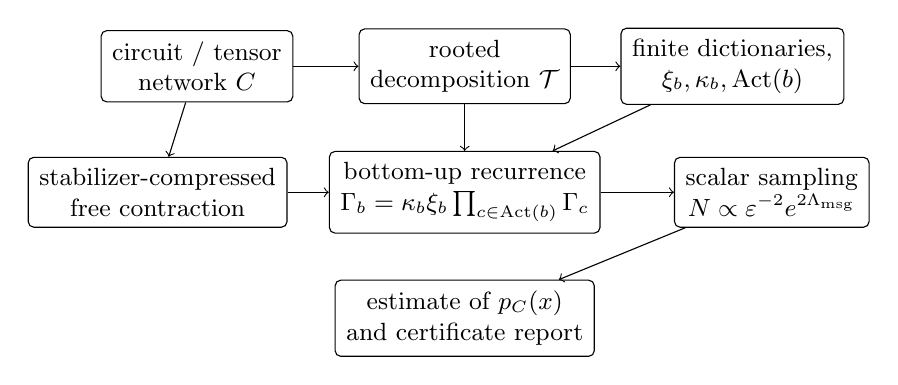
\begin{tikzpicture}[node distance=1.4cm, every node/.style={draw, rounded corners=2pt, align=center, inner sep=4pt, font=\small}]
\node (input) {circuit / tensor\\network \(C\)};
\node[right of=input, xshift=2.0cm] (decomp) {rooted\\decomposition \(\T\)};
\node[right of=decomp, xshift=2.0cm] (cert) {finite dictionaries,\\\(\xi_b,\kappa_b,\Act(b)\)};
\node[below of=decomp, yshift=-0.2cm] (rec) {bottom-up recurrence\\\(\Gamma_b=\kappa_b\xi_b\prod_{c\in\Act(b)}\Gamma_c\)};
\node[right of=rec, xshift=2.5cm] (sample) {scalar sampling\\\(N\propto \eps^{-2}e^{2\Lammsg}\)};
\node[left of=rec, xshift=-2.5cm] (stab) {stabilizer-compressed\\free contraction};
\node[below of=rec, yshift=-0.2cm] (out) {estimate of \(p_C(x)\)\\and certificate report};
\draw[->] (input) -- (decomp);
\draw[->] (decomp) -- (cert);
\draw[->] (cert) -- (rec);
\draw[->] (decomp) -- (rec);
\draw[->] (input) -- (stab);
\draw[->] (stab) -- (rec);
\draw[->] (rec) -- (sample);
\draw[->] (sample) -- (out);
\end{tikzpicture}
\caption{SLMS certificate and scalar-estimation pipeline. The active-child recurrence is a junction-tree-style collect recurrence equipped with stabilizer compression and certified local quasiprobability costs.}
\label{fig:slms-pipeline}
\end{figure}

\subsection{Inputs and message objects}

Figure~\ref{fig:slms-pipeline} summarises the pipeline from input network and decomposition through the active-child recurrence to the scalar sampler. The inputs are:
\begin{itemize}[leftmargin=1.2cm]
\item a circuit or tensor network \(C\) and output event \(x\);
\item a rooted tree decomposition \(\T=(T,\beta)\);
\item an effective-boundary certificate giving \(\weff\);
\item a resource assignment \(\alpha:\R(C)\to V(T)\);
\item local free-tensor decompositions and bag costs \(\xi_b\);
\item certified local coefficient-map norm factors \(\kappa_b\ge 1\);
\item active-child sets \(\Act(b)\subseteq\ch(b)\);
\item an additive error \(\eps>0\) and failure probability \(\delta\in(0,1)\).
\end{itemize}

A message object emitted by a bag \(b\) contains:
\begin{itemize}[leftmargin=1.2cm]
\item the active boundary index set and dense dimension \(D_b\le 2^{\weff}\);
\item a stabilizer/free symbolic representation for the compressed boundary degrees of freedom;
\item a dense table for active boundary entries when needed;
\item the certified burden \(\Gamma_b\);
\item the local sampling distribution over the bag expansion and active child representatives.
\end{itemize}

\subsection{Scalar versus table estimation}

The main theorem analyzes scalar root estimation. In this mode SLMS samples a complete active quasiprobability assignment along the certified recurrence and contracts the corresponding free/stabilizer network to one scalar estimator for \(p_C(x)\). The second moment is bounded by the square of the relevant \(\ell_1\) message cost, hence by \(\exp(2\Lammsg)\).

An implementation may instead estimate intermediate active-boundary message tables entrywise. Then each table has dimension \(D_b\le 2^{O(\weff)}\), each entry needs its own accuracy budget, and a union bound or deterministic error-propagation argument is required over all table entries and all bags. These costs are the source of the \(2^{O(\weff)}\) factor in the theorem. The paper uses scalar estimation for the proof statement and table estimation as an implementation option.

\subsection{Pseudocode}

\begin{center}
\fbox{\begin{minipage}{0.93\linewidth}
\textbf{SLMS: Separator-Local Magic Simulator}

\vspace{0.4em}
\textbf{Input:} \(C,x,\T,\alpha,\{\xi_b\},\{\kappa_b\},\{\Act(b)\},\weff,\eps,\delta\).

\textbf{Output:} Estimate \(\widehat p\) of \(p_C(x)\).

\begin{enumerate}[leftmargin=1.0cm]
\item Verify the contraction graph and the rooted tree decomposition for the scalar \(p_C(x)\).
\item Compress free stabilizer regions and record active boundary dimensions \(D_b\le 2^{\weff}\).
\item For each bag \(b\), form a certified local quasiprobability expansion of cost \(\xi_b\).
\item Compute message burdens bottom-up:
\[
\Gamma_b\leftarrow \kappa_b\xi_b\prod_{c\in\Act(b)}\Gamma_c .
\]
\item Repeat \(N=O(\eps^{-2}\exp(2\Lammsg)\log(1/\delta))\) scalar samples:
\begin{enumerate}[label*=\arabic*.]
\item sample only the local bag expansions and active child representatives appearing in the certified recurrence;
\item treat inactive child messages as deterministic inputs already marginalized at their parent bags;
\item contract the sampled free network using stabilizer compression and dense active boundary dimension at most \(2^{O(\weff)}\);
\item return one signed scalar estimator for \(p_C(x)\).
\end{enumerate}
\item Aggregate the scalar samples, for example by median-of-means, and return \(\widehat p\) with its confidence interval.
\end{enumerate}
\end{minipage}}
\end{center}

\subsection{Certification procedures}
\label{sec:certification}

The theorem is certificate-based, but the certificates are explicit finite checks. For finite tensor networks of bounded local dimension, the following procedures give checkable sufficient conditions. They may be conservative: failing a check means that the child or boundary is marked active, not that the circuit is hard.

\paragraph{Free-region detection.}
Build the induced subgraph on tensors labelled free: stabilizer states, Clifford maps, Pauli effects, computational-basis stochastic maps, and previously certified free mixtures. Connected components of this subgraph are candidate free regions. Boundary legs incident to resource tensors or active child messages are recorded as active legs; all other stabilizer boundary data are stored symbolically.

\paragraph{Effective-width upper bound.}
For each separator \(e\), compute the dense boundary dimension before compression, \(D_e^{\mathrm{TN}}\). Then remove boundary degrees of freedom that the free-region certificate represents purely by stabilizer tableaux, affine symplectic constraints, or normalized classical stochastic stabilizer messages. The remaining dense dimension \(D_e^{\mathrm{act}}\) gives
\[
\weff\le \max_e \log_2 D_e^{\mathrm{act}}.
\]
If the symbolic compression check fails, set \(D_e^{\mathrm{act}}=D_e^{\mathrm{TN}}\).

\paragraph{Inactive-child marginalization check.}
For a child \(c\) of \(b\), form the local map that contracts the message from \(c\) with the tensors at \(b\) that consume the child boundary, while leaving only the outgoing active boundary of \(b\) open. The child can be declared inactive if this map sends every normalized free representative in the certified child message class to a normalized free message or to a deterministic dense active-boundary table with certified \(\ell_1\) cost at most one. For constant-size boundaries this can be checked by enumerating stabilizer extreme points; for larger classical stochastic boundaries it reduces to checking nonnegative column sums.

\paragraph{Local \(\ell_1\)-nonexpansiveness.}
Represent the local contraction map, restricted to the finite list of free representatives appearing in the local and active-child decompositions, as a matrix \(L_b\) from coefficient vectors to outgoing message coefficients. A sufficient certificate is
\[
\norm{L_b}_{1\to 1}=\max_j\sum_i |(L_b)_{ij}|\le 1.
\]
If \(\norm{L_b}_{1\to 1}=L_b^\ast>1\), set \(\kappa_b=L_b^\ast\). If the norm is not certified, the conservative response is to mark the relevant child messages active or merge the local region into a larger certified bag.

\paragraph{Automatic active-child selection.}
Process bags bottom-up. For each child \(c\), attempt the inactive-child marginalization check. If it succeeds, set \(c\notin\Act(b)\). If it fails, set \(c\in\Act(b)\). This greedy rule gives a valid certificate when all local checks pass. It may not minimize \(\Lammsg\), since a globally better certificate may require a different decomposition or local normalization.

\begin{center}
\fbox{\begin{minipage}{0.93\linewidth}
\textbf{CERTIFY-LM: Conservative Local Marginalizability Certification}
\begin{enumerate}[leftmargin=1.0cm]
\item Label tensors as free or resource and identify connected free regions.
\item For each separator, compute \(D_e^{\mathrm{TN}}\) and a certified active dimension \(D_e^{\mathrm{act}}\).
\item For each bag \(b\), compute or import a local free-tensor quasiprobability expansion and cost \(\xi_b\).
\item For each child \(c\in\ch(b)\), run the inactive-child marginalization check.
\item Set \(\Act(b)\) to the children whose check fails.
\item For each bag, compute a certified \(1\to1\) norm factor \(\kappa_b\).
\item Return \(\weff\), \(\{\xi_b\}\), \(\{\kappa_b\}\), \(\{\Act(b)\}\), and \(\Lammsg\).
\end{enumerate}
\end{minipage}}
\end{center}

\subsection{Error allocation}

For a proof-level implementation, assign each message an entrywise accuracy
\[
\eta_b=\Theta\!\left(\frac{\eps}{\poly(|T|)2^{O(\weff)}}\right)
\]
and failure probability \(\delta_b=\delta/\poly(|T|)\). The certified local coefficient-norm factors in Definition~\ref{def:lm-network} are already included in \(\Gamma_b\), so message errors accumulate by at most the polynomial factor in the number of bags and active boundary dimension. This optional message-table mode gives the same dependence on \(\eps\), \(\delta\), \(\weff\), and the explicit sampling factor \(\exp(2\Lammsg)\) as the scalar theorem in Section~\ref{sec:main-theorem}, with additional implementation constants from table storage and error propagation.

\subsection{Baselines}

\begin{center}
\begin{tabular}{lll}
\toprule
Method & Dominant exponential & When it is relevant \\
\midrule
Dense tensor-network contraction & \(2^{O(\wTN)}\) & arbitrary tensors \\
Global quasiprobability sampling & \(\exp(2\Lambda_{\mathrm{glob}})\) & low total magic \\
Naive hybrid & \(2^{O(\weff)}\exp(2\Lambda_{\mathrm{glob}})\) & no local marginalization \\
SLMS (this paper) & \(2^{O(\weff)}\exp(2\Lammsg)\) & locally marginalizable networks \\
\bottomrule
\end{tabular}
\end{center}

The SLMS row is not automatically better than dense contraction. It is useful only when stabilizer compression gives \(\weff\ll\wTN\), or when the active-child recurrence gives \(\Lammsg\ll\Lambda_{\mathrm{glob}}\), or both. The scalar Monte Carlo variance bound gives the explicit sampling dependence \(\exp(2\Lammsg)\).

\section{Main Theorem and Separations}
\label{sec:main-theorem}

This section proves the main theorem for locally marginalizable resource-decomposition networks. The result is not a theorem for arbitrary compositional circuits. The broader separator-factorization principle is isolated as Conjecture~\ref{conj:general-separator}.

\begin{theorem}[Free-region compression]
\label{thm:free-compression}
Let \(H\) be a connected free stabilizer subnetwork whose outgoing boundary has certified effective active dimension at most \(2^{\weff}\). Then the boundary message of \(H\) can be computed or represented in time \(\poly(|H|)2^{O(\weff)}\), using stabilizer data for the free boundary degrees of freedom, without increasing any quasiprobability cost.
\end{theorem}

\begin{proof}
Free stabilizer tensors are closed under tensor product, composition, Clifford conjugation, Pauli measurement, and partial trace. A connected free subnetwork therefore represents a stabilizer state, effect, channel, or affine stabilizer relation on its boundary. Standard stabilizer-tableau simulation gives a symbolic representation in time polynomial in \(|H|\). If the certified representation leaves an active dense boundary factor of dimension \(D\le 2^{\weff}\), extracting or updating the dense active table costs \(D^{O(1)}=\allowbreak 2^{O(\weff)}\). No resource expansion is introduced, so the quasiprobability cost is unchanged.
\end{proof}

\begin{lemma}[Local quasiprobability expansion]
\label{lem:bag-expansion}
Let \(b\) be a bag with assigned resource tensors \(\R_b\). If each \(A\in\R_b\) admits a free-tensor expansion \(A=\sum_j a_{A,j}F_{A,j}\) of cost \(\xi(A)\), then the product of resource tensors assigned to \(b\) admits a free-tensor expansion of cost at most
\[
\xi_b=\prod_{A\in\R_b}\xi(A).
\]
If an optimized joint expansion is supplied, \(\xi_b\) may be replaced by its certified joint \(\ell_1\) cost.
\end{lemma}

\begin{proof}
Taking the tensor product or local composition of the individual expansions gives
\[
\prod_{A\in\R_b}A
=\sum_{(j_A)}
\left(\prod_{A\in\R_b}a_{A,j_A}\right)
\left(\prod_{A\in\R_b}F_{A,j_A}\right).
\]
The free tensor class is closed under the local compositions used inside a bag. The \(\ell_1\) cost is bounded by
\[
\sum_{(j_A)}\prod_A |a_{A,j_A}|
=\prod_A\sum_{j_A}|a_{A,j_A}|
=\prod_A\xi(A).
\]
\end{proof}

\begin{stackdefinition}[Message burden]
\label{def:constructive-burden}
For a locally marginalizable network, define
\[
\Gamma_b=\kappa_b\xi_b\prod_{c\in\Act(b)}\Gamma_c
\]
from leaves to root, and
\[
\Lammsg(C,\T)=\max_{b\in V(T)}\log\Gamma_b .
\]
\end{stackdefinition}

\begin{lemma}[Message expansion and second-moment recurrence]
\label{lem:message-recurrence}
For every bag \(b\) in a locally marginalizable resource-decomposition network, the outgoing message \(M_b\) has an expansion
\[
M_b=\sum_{\omega\in\Omega_b} q_b(\omega) F_{b,\omega}
\]
where \(F_{b,\omega}\) are normalized free representatives on the certified active boundary, and
\[
\sum_{\omega\in\Omega_b}|q_b(\omega)|\le \Gamma_b .
\]
Consequently a single-sample unbiased estimator of any normalized entry or normalized linear functional of \(M_b\) has second moment at most \(\Gamma_b^2\).
\end{lemma}

\begin{proof}
Proceed by induction from the leaves. For a leaf, the only unresolved quasiprobability choices are those in the local bag expansion. Lemma~\ref{lem:bag-expansion} gives an expansion of \(\ell_1\) cost at most \(\xi_b\), and the certified local coefficient map increases this by at most \(\kappa_b\). Thus the outgoing cost is at most \(\Gamma_b\).

For an internal bag \(b\), inactive child messages are, by local marginalizability, already consumed by local marginalization maps and enter as normalized deterministic free or active-boundary messages. They therefore contribute no quasiprobability coefficient to the outgoing expansion. Each active child \(c\in\Act(b)\) has, by the induction hypothesis, an expansion of \(\ell_1\) cost at most \(\Gamma_c\). Tensoring the local bag expansion with the active child expansions gives coefficient \(\ell_1\) norm at most
\[
\xi_b\prod_{c\in\Act(b)}\Gamma_c .
\]
The local contraction map has certified coefficient norm at most \(\kappa_b\) on normalized free representatives and maps free representatives to normalized free representatives on the outgoing certified boundary. Hence the outgoing expansion has \(\ell_1\) norm at most
\[
\kappa_b\xi_b\prod_{c\in\Act(b)}\Gamma_c=\Gamma_b .
\]

Sampling \(\omega\) with probability \(|q_b(\omega)|/\sum_\omega |q_b(\omega)|\) and returning the signed representative gives an unbiased estimator. Normalization bounds the squared magnitude of any entry or normalized linear functional by one, so the second moment is bounded by \((\sum_\omega |q_b(\omega)|)^2\le \Gamma_b^2\).
\end{proof}

\begin{theorem}[SLMS scalar simulation theorem]
\label{thm:main}
Let \(C\) be a compositional circuit or tensor network whose scalar output probability \(p_C(x)\) is represented by a locally marginalizable resource-decomposition network over a rooted tree decomposition \(\T\). Let \(\weff\) be the certified effective stabilizer-compressed width and \(\Lammsg(C,\T)\) the message burden. Then SLMS estimates \(p_C(x)\) to additive error \(\eps\) with failure probability at most \(\delta\) in time
\[
\wt{O}\!\left(
\poly(|C|)
\eps^{-2}\log(1/\delta)
2^{O(\weff)}
\exp(2\Lammsg(C,\T))
\right).
\]
\end{theorem}

\begin{proposition}[SLMS as a checkable sufficient certificate]
\label{prop:checkable-certificate}
Fix a rooted decomposition \(\T\), finite free dictionaries for every local tensor type, local resource assignments, local expansion coefficients, local coefficient-map matrices, and active-child declarations. Suppose all local tensors have bounded arity and the supplied free dictionaries have size at most polynomial in \(|C|\). Then the following are checkable in time polynomial in the certificate size:
\begin{enumerate}[leftmargin=1.2cm]
\item whether each local expansion has the claimed \(\ell_1\) cost \(\xi_b\);
\item whether each local coefficient map has certified norm at most \(\kappa_b\) in the chosen finite basis;
\item whether every inactive child is accompanied by a local marginalization certificate producing a deterministic free or bounded active-boundary message;
\item the values \(\Gamma_b\), \(\Lammsg\), \(\Lambda_{\mathrm{glob}}\), and the exponent proxy \(\weff+2\Lammsg\).
\end{enumerate}
If these checks pass, Theorem~\ref{thm:main} applies. If a check fails, the conclusion is only that this certificate fails; it is not evidence that the circuit is classically hard.
\end{proposition}

\begin{proof}
The local expansions and coefficient-map norm bounds are finite linear-algebra checks in the supplied dictionaries. The inactive-child condition is checked by the supplied marginalization certificates and the syntactic/free-region tests described in Section~\ref{sec:algorithm} and Appendix~\ref{app:certification}. The recurrence for \(\Gamma_b\) is a single bottom-up traversal of \(\T\). The claimed running time is polynomial in the explicitly supplied finite certificate because no optimization over decompositions, dictionaries, or active-child sets is required. The final implication is exactly Theorem~\ref{thm:main}.
\end{proof}

\begin{remark}[Explicit factor of 2 in the exponent]
\label{rem:factor-two}
The sampling cost is governed by the second moment of the scalar estimator. With the convention \(\Lammsg=\max_b\log\Gamma_b\), Lemma~\ref{lem:message-recurrence} gives second moment at most \(\Gamma_r^2\le\exp(2\Lammsg)\), so the sample count scales as \(\exp(2\Lammsg)/\eps^2\). Concrete sample-count estimates use the explicit \(\exp(2\Lammsg)\) form, as in Section~\ref{sec:algorithm}.
\end{remark}

\paragraph{Non-asymptotic accounting form.}
The \(\widetilde O\)-statement isolates the asymptotic dependence on \(\weff\) and \(\Lammsg\). For implementation accounting it is useful to write
\[
T_{\mathrm{total}}
\le C_{\mathrm{cert}}+
N\,C_{\mathrm{sample}},
\qquad
N=
O\!\left(\eps^{-2}\exp(2\Lammsg)\log(1/\delta)\right),
\]
where \(C_{\mathrm{cert}}\) is the time to verify the supplied finite dictionaries, local expansions, \(\kappa_b\) bounds, active-child declarations, and effective-width certificates. The per-sample cost satisfies
\[
C_{\mathrm{sample}}
\le \poly(|C|)\,2^{c\weff}\,D_{\mathrm{dict}}^{c'}\,d_{\max}^{c''},
\]
for constants depending on the fixed local tensor model, maximum local dictionary size \(D_{\mathrm{dict}}\), and maximum local index dimension \(d_{\max}\). The experiment section reports the exponent proxy \(\weff+2\Lammsg\) because this is the certificate-visible part before backend-dependent constants and dictionary sizes are optimized.

\paragraph{Scalar versus table estimation.}
The theorem is stated for estimating the root scalar \(p_C(x)\). One can also estimate intermediate active-boundary message tables entrywise, but then the table dimension \(D_b\le 2^{O(\weff)}\), per-entry accuracy, and union bounds must be included explicitly. The proof below uses the scalar mode: a sample fixes a complete active quasiprobability assignment generated by the certified recurrence, contracts the remaining free/stabilizer network symbolically with active boundary dimension bounded by \(2^{O(\weff)}\), and returns a single unbiased scalar estimator.

\begin{proof}
By Lemma~\ref{lem:message-recurrence}, the root message, after applying the final effect for the event \(x\), has a scalar quasiprobability expansion with \(\ell_1\) cost at most \(\Gamma_r\), where \(r\) is the root bag. Sampling from the absolute values of the active local and active-child coefficients in the recurrence and returning the corresponding signed free contraction gives an unbiased estimator of \(p_C(x)\). Inactive child subtrees contribute deterministic normalized free or active-boundary messages by local marginalizability, so their resource coefficients do not enter the sampled root assignment.

For each sampled assignment, Theorem~\ref{thm:free-compression} contracts the remaining free/stabilizer regions symbolically and handles any dense active boundary with dimension bounded by \(2^{O(\weff)}\). Thus a single sample costs \(\poly(|C|)2^{O(\weff)}\). The scalar estimator has second moment at most
\[
\Gamma_r^2\le \left(\max_b\Gamma_b\right)^2
=\exp(2\Lammsg(C,\T)).
\]
Median-of-means estimation therefore uses
\[
O\!\left(\eps^{-2}\exp(2\Lammsg(C,\T))\log(1/\delta)\right)
\]
samples, up to polynomial factors and the active-boundary contraction cost. Combining these factors gives
\[
\wt{O}\!\left(
\poly(|C|)\eps^{-2}\log(1/\delta)
2^{O(\weff)}
\exp(2\Lammsg(C,\T))
\right).
\]
\end{proof}

\begin{corollary}[Polynomial-time easy regime]
\label{cor:poly}
For a circuit family \(\{C_n\}\), suppose there exist locally marginalizable decompositions \(\T_n\) such that
\[
\weff(\T_n)+2\Lammsg(C_n,\T_n)=O(\log n),
\]
with bounded local dimension and polynomially describable local certificates. Then output probabilities of \(\{C_n\}\) are additively estimable in randomized polynomial time.
\end{corollary}

\begin{proof}
Substitute the logarithmic bound into Theorem~\ref{thm:main}. The exponential factors become polynomial in \(n\).
\end{proof}

\begin{example}[Constant-boundary separation from global-magic accounting]
\label{prop:improvement}
There is a family of locally marginalizable tree tensor networks \(\{C_n\}\) with \(n\) resource tensors and non-scalar one-bit boundary messages such that
\[
\Lambda_{\mathrm{glob}}(C_n,\T_n)=\Theta(n)
\qquad\text{but}\qquad
\Lammsg(C_n,\T_n)=O(1).
\]
For this pedagogical family, naive global quasiprobability accounting gives exponential overhead in \(n\), while the certified SLMS recurrence gives polynomial overhead. The example is not presented as a state-of-the-art simulation separation.
\end{example}

\begin{proof}
Let each leaf contain one copy of the one-qubit non-stabilizer state
\[
\ket{T}=(\ket0+e^{i\pi/4}\ket1)/\sqrt2 .
\]
The leaf applies the following stabilizer instrument: measure the \(X\) Pauli observable on \(\ket{T}\), write the classical outcome \(y\in\{0,1\}\) into a computational-basis boundary register, and discard the measured qubit. The outgoing leaf message is the one-bit classical stabilizer mixture
\[
\rho_T
=p\,\ket0\!\bra0+(1-p)\ket1\!\bra1,
\qquad
p=\frac{1+1/\sqrt2}{2}.
\]
This message is not a scalar; it is a constant-size boundary distribution that will be combined by the rest of the tree.

Each internal node takes two incoming one-bit classical boundary registers, prepares a fresh \(\ket0\) target, applies two CNOT gates into the target, and discards the two inputs. Thus the internal node computes the XOR of the two child bits and emits a one-bit classical stabilizer message. At the root, measure whether the final parity bit is \(0\). The resulting output probability is the even-parity probability of \(n\) independent biased bits, for example
\[
p_{\mathrm{even}}=\frac{1+(2p-1)^n}{2}
\]
for a balanced tree with \(n\) leaves.

Let \(\xi_T>1\) be any certified free-tensor quasiprobability cost for the local \(\ket{T}\) resource representation. Then \(\xi_b=\xi_T\) for leaf bags and \(\xi_b=1\) for internal bags, so
\[
\Lambda_{\mathrm{glob}}=\sum_b\log\xi_b=n\log\xi_T=\Theta(n).
\]
However each \(\ket{T}\) resource is locally consumed by the Pauli measurement instrument before its message crosses the first separator. The outgoing one-bit boundary message \(\rho_T\) is a free classical stabilizer mixture of \(\ell_1\) cost one, and the local maps have \(\kappa_b=1\). Hence all children can be declared inactive after the leaf marginalization, and every internal XOR node is free. The recurrence gives \(\Gamma_b=\xi_T\) at leaves and \(\Gamma_b=1\) at internal bags, so \(\Lammsg=\log\xi_T=O(1)\). The effective active boundary is one classical bit, so \(\weff=O(1)\). SLMS computes or estimates the leaf boundary distributions locally and combines them through free XOR messages in polynomial time, while a sampler that expands all \(n\) \(\ket{T}\) resources globally pays \(\xi_T^{\Theta(n)}\) overhead.
\end{proof}

\begin{example}[Path-active separation from global-magic accounting]
\label{prop:path-active-improvement}
There is a family of locally marginalizable tree tensor networks \(\{D_n\}\), with \(n\) leaf-local resource tensors and \(O(\log n)\) additional path resources, for which
\[
\Lambda_{\mathrm{glob}}(D_n,\T_n)=\Theta(n)
\qquad\text{but}\qquad
\Lammsg(D_n,\T_n)=O(\log n).
\]
In this family a nontrivial resource label remains active along one root-to-leaf path, while all off-path leaf resources are locally marginalized before joining that path.
\end{example}

\begin{proof}
Let \(n=2^h\) and use a balanced binary tree of height \(h\). Put one \(\ket T\)-type resource of certified cost \(\xi_T>1\) at every leaf. The off-path leaves use the same local Pauli-measurement gadget as in Example~\ref{prop:improvement}, so each exports a one-bit classical stabilizer boundary message and no unresolved quasiprobability label.

Choose the leftmost root-to-leaf path \(\pi\). Along \(\pi\), add one constant-size resource gadget of certified cost \(\xi_P>1\) at each internal bag. The gadget acts on the current one-bit boundary and is not marginalized until the root; equivalently, in the active-child certificate, the child continuing along \(\pi\) is active at each path bag. The sibling subtree at each path bag is inactive because its resources have already been locally measured into free one-bit messages. All off-path internal composition maps are Clifford XOR maps, as in Example~\ref{prop:improvement}.

The global quasiprobability burden includes the \(n\) leaf costs and \(h\) path costs:
\[
\Lambda_{\mathrm{glob}}
=n\log\xi_T+h\log\xi_P
=\Theta(n).
\]
For the message recurrence, off-path subtrees contribute no active child burden after local marginalization. At a path bag, the only active child is the next child on \(\pi\), and the local multiplicative cost is at most \(\xi_P\), except at the terminal leaf where it is at most \(\xi_T\). Therefore
\[
\max_b \log\Gamma_b
\le \log\xi_T+h\log\xi_P
=O(\log n).
\]
The active boundary is still constant size: one classical or stabilizer-frame bit plus the constant-size path gadget state. Hence \(\weff=O(1)\) for the certified representation. The family separates SLMS from naive global quasiprobability sampling, while also showing a regime in which resource randomness is not merely consumed at independent leaves. It is not, by itself, a separation from dense tensor-network contraction unless the dense width of the chosen circuit family is made large while the stabilizer-compressed width remains constant.
\end{proof}

\begin{proposition}[Parameter separation from dense treewidth bounds]
\label{thm:dense-width-separation}
There is a family of locally marginalizable resource-decomposition networks \(\{G_L\}\), built from an \(L\times L\) stabilizer graph-state core with locally measured non-Clifford leaf gadgets, such that the ordinary dense contraction graph has treewidth
\[
\wTNopt(G_L)=\Theta(L),
\]
while the certified SLMS parameters satisfy
\[
\weff(G_L)=O(1),\qquad
\Lammsg(G_L)=O(1).
\]
The global quasiprobability burden of the attached resource gadgets is \(\Theta(L^2)\). Thus the certified SLMS bound is polynomial for this family, whereas the dense Markov--Shi-style treewidth expression for the uncompressed tensor network has exponential dependence \(2^{\Theta(L)}\).
\end{proposition}

This is only a parameter separation between dense treewidth bounds and stabilizer-compressed separator-local certificates. It is not a lower bound against algorithms that already exploit stabilizer tableau structure, ZX rewriting, focused width, or stabilizer tensor-network representations.

\begin{proof}
Let \(Q_L\) be the \(L\times L\) square grid. The free core prepares the graph state \(\ket{Q_L}\) using \(\ket+\) preparations and controlled-\(Z\) gates on grid edges, and then applies a fixed product of Pauli or computational-basis effects whose probability is the target scalar. This entire core is a stabilizer tensor network.

At each grid vertex attach a constant-size leaf gadget containing one \(\ket T\)-type resource of certified quasiprobability cost \(\xi_T>1\). The gadget is consumed locally by a Pauli measurement or stabilizer instrument and exports only a classical stabilizer mixture or a Pauli-frame bit into the adjacent grid-site tensor. As in Example~\ref{prop:improvement}, this exported message is non-scalar but free after local marginalization. All local coefficient maps have \(\kappa_b=1\).

The dense contraction graph contains the \(L\times L\) grid as a minor after deleting the attached leaf gadgets and suppressing constant-size internal gadget vertices. The treewidth of the square grid is \(\Theta(L)\), and adding constant-size leaf gadgets changes treewidth by at most a constant factor. Hence the optimal dense treewidth-type parameter of the uncompressed contraction graph is \(\wTNopt(G_L)=\Theta(L)\).

For SLMS, first certify the connected graph-state core as one free stabilizer region. Standard tableau simulation represents its boundary and Pauli-frame data using polynomial-size symbolic stabilizer data. Since every attached resource gadget is locally marginalized before its quasiprobability label enters the grid core, no non-stabilizer choice crosses a grid separator. The only dense active data are constant-size local classical bits or the final scalar effect, so \(\weff=O(1)\).

There are \(L^2\) resource gadgets, so
\[
\Lambda_{\mathrm{glob}}=L^2\log\xi_T=\Theta(L^2).
\]
However each gadget is assigned to its own local bag and is inactive before communicating with the stabilizer core. Thus \(\Gamma_b\le \xi_T\) for gadget bags and \(\Gamma_b=1\) for the free core bags, giving \(\Lammsg=O(1)\). The active-child recurrence is the extra ingredient beyond the stabilizer easiness of graph states: it certifies that the locally attached non-Clifford gadgets do not load the grid separators. Theorem~\ref{thm:main} then gives a polynomial certified upper bound. The dense-width comparison is a comparison with the width expression obtained by contracting the original dense tensor network; it is not a lower bound against algorithms that exploit stabilizer tableau structure, ZX simplification, focused width, or stabilizer tensor-network methods.
\end{proof}

\paragraph{Referee caveat.}
An expert may object that the graph-state core is already stabilizer-simulable. This is exactly the point of the construction: dense treewidth is not the right parameter once a large free stabilizer region is represented symbolically. The theorem separates width parameters and simulation upper bounds for certified representations; it does not establish a complexity-theoretic lower bound against stabilizer-aware classical algorithms.

\begin{corollary}[Polynomial certified simulation despite superlogarithmic dense width]
\label{cor:dense-width-bound-separation}
Let \(\{C_n\}\) be a locally marginalizable family with polynomially describable certificates such that
\[
\wTNopt(C_n)=\omega(\log n),
\qquad
\weff(C_n)+2\Lammsg(C_n,\T_n)=O(\log n).
\]
Then Theorem~\ref{thm:main} gives a randomized polynomial-time additive simulation bound for the certified representation, while the dense treewidth expression \(2^{\Theta(\wTNopt(C_n))}\) is superpolynomial. This compares parameterized upper bounds only and does not rule out other classical algorithms.
\end{corollary}

\begin{proof}
The SLMS statement follows from Corollary~\ref{cor:poly}. Since \(\wTNopt(C_n)=\omega(\log n)\), the dense-width exponential expression \(2^{\Theta(\wTNopt(C_n))}\) grows faster than any polynomial in \(n\). The claim is only about the dense treewidth cost expression.
\end{proof}

\begin{proposition}[Non-improvement over dense treewidth in the uncompressed regime]
\label{prop:non-improvement}
If \(\weff=\wTN\) for a decomposition and \(\Lammsg(C,\T)>0\), then the SLMS bound is not asymptotically better than the ordinary dense tensor-network contraction bound \( \wt{O}(\poly(|C|)2^{O(\wTN)}) \) on the basis of width alone.
\end{proposition}

\begin{proof}
With \(\weff=\wTN\), Theorem~\ref{thm:main} gives the dense-width factor \(2^{O(\wTN)}\) multiplied by the additional nonnegative factor \(\exp(2\Lammsg)\). Dense tensor-network contraction does not pay this magic factor because it contracts the original tensors directly. Thus any advantage of SLMS in this case must come from constants, implementation details, reuse of local marginalizations, or comparison to global-magic sampling, not from an asymptotic improvement over the Markov--Shi-style width bound.
\end{proof}

\begin{conjecture}[General separator-local factorization]
\label{conj:general-separator}
For broader compositional tensor networks beyond the locally marginalizable class, there may exist message estimators whose variance is controlled by resource tensors that remain genuinely active across each separator, rather than by the global product of all resource costs. An explicit version of this conjecture requires a concrete estimator, a computable separator burden, and a proof of unbiasedness and second-moment control.
\end{conjecture}

\section{Specialization to QDisCoCirc and lambeq-Style Circuits}
\label{sec:qnlp}

\subsection{Grammar-induced contraction graphs}

In lambeq-style QNLP, a sentence is parsed into a grammatical derivation or string diagram. The diagram is rewritten and mapped through an ansatz to a tensor network or quantum circuit \citep{KartsaklisEtAl2021}. Noun, sentence, and relation types become wires or registers; words and grammatical reductions become tensors, effects, or circuit fragments. The contraction graph \(G_C\) is obtained by placing vertices at word tensors, cups/effects, ansatz blocks, and measurement effects, with edges corresponding to contracted grammatical wires and circuit wires.

For pregroup-like sentence diagrams, the induced graphs are often close to trees or low-width series-parallel structures after diagram simplification. This explains why many small QNLP models are accessible to tensor-network contraction. The main theorem refines the statement only for circuits that also satisfy local marginalizability: non-Clifford word or phrase modules must be locally compressed, measured, or marginalized before their unresolved quasiprobability choices propagate through many separators. General trained lambeq ans\"atze with continuous rotations, hardware-efficient entanglers, or non-Clifford phrase-level relation tensors may violate this condition.

\subsection{QDisCoCirc}

QDisCoCirc extends sentence-level composition to text circuits whose vertices represent entities, predicates, discourse updates, and question-answering effects \citep{LaakkonenMeichanetzidisCoecke2024}. Such circuits may introduce more entangling structure than a single sentence parse. Some instances may satisfy the locally marginalizable condition, especially when resourceful lexical modules are consumed inside sentence or phrase subtrees. Other instances may violate it, for example when non-Clifford discourse updates remain coherent across document-level separators.

\begin{proposition}[QNLP specialization for locally marginalizable circuits]
\label{prop:qdiscocirc-specialization}
Let \(C_D\) be a QDisCoCirc or lambeq-style circuit obtained from a composition diagram \(D\). Suppose:
\begin{enumerate}[leftmargin=1.2cm]
\item the diagram-to-circuit translation produces a bounded-degree contraction graph \(G_{C_D}\);
\item a rooted tree decomposition \(\T_D\) and stabilizer-compressed boundary certificate of width \(\weff\) are supplied;
\item non-Clifford word, relation, or discourse-update tensors admit local quasiprobability expansions with certified costs \(\xi_b\);
\item the active-child and local marginalization conditions of Definition~\ref{def:lm-network} hold.
\end{enumerate}
Then output probabilities for \(C_D\) obey the scalar SLMS bound of Theorem~\ref{thm:main} with burden \(\Lammsg(C_D,\T_D)\).
\end{proposition}

\begin{proof}
The diagram-to-circuit translation supplies the tensor network and contraction graph. The decomposition, effective-boundary certificate, resource assignment, local expansions, and active-child sets instantiate a locally marginalizable resource-decomposition network. Theorem~\ref{thm:main} then applies.
\end{proof}

\subsection{A certified grammar-tree family}

\begin{proposition}[Certified grammar-tree family]
\label{prop:certified-lambeq-family}
Fix a bounded-arity pregroup or context-free grammar fragment. Fix a constant local dimension \(d_\tau\) for every grammatical type \(\tau\), and allow only a bounded number of noun, sentence, relation, and feature wires across every grammar reduction. Consider lambeq-style sentence circuits in which:
\begin{enumerate}[leftmargin=1.2cm]
\item the parse diagram is a rooted tree with word modules at leaves and grammatical reductions at internal nodes;
\item the allowed free tensors are cups and evaluations, computational-basis effects, copying or parity maps on classical feature bits, Clifford relation tensors, and classical stochastic maps whose coefficient norm is certified;
\item each resource word or phrase module is constant size, has certified free-tensor quasiprobability \(\ell_1\) cost at most \(\xi_\star\), and either is locally consumed before phrase composition or exports a bounded stabilizer-frame or classical feature message;
\item optionally, one distinguished bounded-size semantic feature is allowed to remain active along a single root-to-leaf path, with at most \(O(1)\) resource cost per bag on that path and all sibling phrase subtrees locally marginalized;
\item all local coefficient norm factors obey \(\kappa_b\le \kappa_\star=O(1)\).
\end{enumerate}
Then the induced circuits are locally marginalizable with respect to the parse-tree decomposition. If no distinguished path is active, then \(\weff=O(1)\) and \(\Lammsg=O(1)\). If one distinguished path is active in a balanced \(n\)-word parse tree, then \(\weff=O(1)\) and \(\Lammsg=O(\log n)\). In both cases Theorem~\ref{thm:main} applies.
\end{proposition}

\begin{proof}
Use the parse tree as the rooted decomposition. Bounded grammar arity and bounded type dimension imply that each separator carries only a bounded number of grammatical and feature wires before stabilizer compression. The grammatical reductions and phrase-composition maps are free by assumption, so they can be represented by stabilizer, affine, or classical stochastic data.

For a resource word module, the non-Clifford tensor is assigned to the corresponding leaf bag. Its supplied quasiprobability expansion has cost at most \(\xi_\star\). The subsequent stabilizer instrument consumes the resource locally and exports a bounded classical stabilizer feature message, so the inactive-child marginalization check succeeds before the first phrase separator. Thus leaf-local resource labels do not multiply into ancestor messages.

If no distinguished feature is active, every internal child can be declared inactive after its phrase message is converted into a bounded free feature message. The recurrence gives \(\Gamma_b\le \kappa_\star\xi_\star\) at resource leaves and \(O(1)\) at free internal bags, so \(\Lammsg=O(1)\). If one distinguished feature remains unresolved along a root-to-leaf path, the active-child set contains only the child continuing that path. The recurrence then multiplies only the \(O(1)\) costs on that path, giving \(\Lammsg=O(\log n)\) for a balanced parse tree. In both cases the dense active boundary dimension is bounded by the fixed grammar and feature dimensions, so \(\weff=O(1)\).
\end{proof}

The construction is deliberately restricted. It shows that the hypotheses of Proposition~\ref{prop:qdiscocirc-specialization} are checkable on a lambeq-shaped family, not that practical trained lambeq circuits or arbitrary language tasks satisfy the theorem. It is best viewed as a warm-start or easy-subclass certificate: the same parse-tree structure can be used to record where a more expressive ansatz first fails local marginalizability.

SLMS is best viewed as a dequantisation diagnostic for structured QNLP ans\"atze: it identifies when a proposed circuit family remains classically easy under the chosen certificate. A high certificate pass rate on Clifford-like or discretized warm-start instances would not imply practical quantum advantage; it would instead indicate that those instances remain in an easy regime. A low pass rate would not prove hardness, but it would identify where continuous rotations, entangling phrase tensors, or discourse-level updates obstruct the local-marginalization certificate.

\subsection{A synthetic lambeq-style diagnostic case}

Consider the pregroup-style sentence pattern
\[
\text{noun}\quad \text{adverb}\quad \text{transitive verb}\quad \text{noun},
\]
with a bounded parse tree whose reductions evaluate the noun wires against the verb type and pass one sentence wire to the root. Let the two noun word modules be free stabilizer preparations. Let the adverb and verb modules each contain one constant-size non-Clifford lexical gadget with certified costs \(\xi_{\mathrm{adv}}\) and \(\xi_{\mathrm{verb}}\). Inside each lexical module, the resource is measured by a Pauli effect and the outcome is written into a bounded computational-basis feature register. The grammatical reductions, cups, and feature-composition maps are free Clifford or classical affine tensors.

Use the parse-tree decomposition with resource assignments at the adverb and verb leaf bags. If both lexical resources are locally consumed before phrase composition, the global burden is
\[
\Lambda_{\mathrm{glob}}
=\log\xi_{\mathrm{adv}}+\log\xi_{\mathrm{verb}},
\]
whereas the active-child recurrence has no active internal child after the lexical marginalizations and gives
\[
\Lammsg
=\max\{\log\xi_{\mathrm{adv}},\log\xi_{\mathrm{verb}}\}+O(\log\kappa_\star).
\]
The effective boundary width is bounded by the fixed sentence type dimension and the bounded feature register size, so \(\weff=O(1)\).

A one-path variant leaves the verb sentiment feature unresolved until the sentence root while locally marginalizing the adverb feature into a free modifier message. Then the child on the verb-to-root path is active, all sibling phrase subtrees are inactive, and
\[
\Lammsg
\le \log\xi_{\mathrm{verb}}+O(\log\kappa_\star)
\]
for this constant-depth diagnostic. In a balanced sentence family with the same rule applied along one distinguished semantic path, the same calculation gives the \(O(\log n)\) active-path behavior of Proposition~\ref{prop:certified-lambeq-family}.

This is a diagnostic calculation, not empirical lambeq data. Generic trained lambeq ans\"atze with continuous rotations, trainable non-Clifford layers at phrase boundaries, or high-level entangling relation tensors may fail the certificate. The point of the example is to show how \(\Lambda_{\mathrm{glob}}\), \(\Lammsg\), \(\weff\), and active-child declarations are checked on a concrete grammar-shaped circuit family.

\begin{openproblem}[Separator burden in QDisCoCirc hardness constructions]
\label{conj:qdiscocirc-nonvacuity}
Determine whether explicit QDisCoCirc hardness constructions force large dense width, large effective width, large message burden, or failure of local marginalizability for natural decompositions. Resolving this requires mapping the construction to lower bounds on \(\weff+2\Lammsg\) or to a formal obstruction to local marginalization.
\end{openproblem}

The conditional BQP-hardness result of Laakkonen, Meichanetzidis, and Coecke~\citep{LaakkonenMeichanetzidisCoecke2024} does not by itself resolve this open problem. It shows that certain compositional text-processing tasks can encode hard quantum computation under explicit assumptions. It does not directly imply lower bounds on treewidth, stabilizer-compressed width, or separator-local message burden.

\subsection{Resource placement patterns}

The framework distinguishes several patterns that global resource counts conflate.

\begin{itemize}[leftmargin=1.2cm]
\item \emph{Leaf-local lexical magic.} Non-Clifford parameters occur inside word modules near leaves of a parse tree. If each lexical module is contracted to a bounded free or dense boundary before phrase composition, \(\Lammsg\) can remain small.

\item \emph{Phrase-boundary magic.} Non-Clifford tensors sit at phrase-composition maps. These tensors may be active across phrase separators and can increase \(\Lammsg\) even if their number is modest.

\item \emph{Discourse-level magic.} Non-Clifford updates connect sentence or paragraph modules. These are likely to load high-level separators and may violate local marginalizability.

\item \emph{Distributed weak magic.} Many low-cost resource tensors are spread across the graph. Whether this is easy depends on whether their effects can be marginalized locally or whether they coherently combine across separators.
\end{itemize}

\subsection{Interpretation}

The specialization does not imply that QNLP circuits are quantum-advantaged or classically hard. It gives a diagnostic and algorithmic vocabulary. A certified lambeq-style circuit with low \(\weff\) and low \(\Lammsg\) is classically simulable by the present theorem. A general lambeq or QDisCoCirc circuit outside the locally marginalizable class is not covered by the theorem; it must be analyzed either by ordinary tensor-network width, global magic methods, focused-width or ZX-inspired methods, stabilizer tensor-network methods, or an extension of Conjecture~\ref{conj:general-separator}.

\section{Benchmark Protocol}
\label{sec:benchmarks}

This section reports a minimal synthetic accounting benchmark. These are not quantum-circuit simulations and are not hardware experiments. They only validate the bookkeeping behavior of \(\Lambda_{\mathrm{glob}}\), \(\Lammsg\), dense-width proxies, and SLMS exponent proxies on generated tree/resource instances.

\subsection{Synthetic accounting benchmarks}

The first benchmark layer is purely combinatorial. It generates rooted trees, assigns local costs \(\xi_b\), local norm factors \(\kappa_b\), width proxies, and local marginalizability flags, then computes:
\[
\Lambda_{\mathrm{glob}},\qquad
\max_b\log\xi_b,\qquad
\Lambda_{\mathrm{path}},\qquad
\Lambda_{\mathrm{subtree}},\qquad
\Lammsg,\qquad
\weff+2\Lammsg .
\]
This validates the behavior of the burden definitions before any quantum-circuit backend is implemented.

The accounting implementation consists of:
\begin{itemize}[leftmargin=1.2cm]
\item \texttt{benchmarks/generate\_tree\_resource\_network.py}, which generates balanced binary trees, chains, star-like trees, and random grammar-like trees with controlled resource placement modes;
\item \texttt{benchmarks/compute\_synthetic\_burdens.py}, which computes global, bag, path, subtree, and recurrence-based message burdens from the generated CSV file;
\item \texttt{benchmarks/certify\_synthetic\_lm.py}, which applies a conservative synthetic local-marginalizability certificate and generates active-child sets.
\item \texttt{benchmarks/run\_examples.sh} and \texttt{benchmarks/plot\_burdens.py}, which generate the synthetic examples below, write \texttt{benchmarks/results/summary.csv}, and produce two dependency-free SVG plots.
\end{itemize}

\subsection{Synthetic accounting outputs}

Running \texttt{benchmarks/run\_examples.sh} produces the following accounting table. Values are natural-log cost proxies. The column \(\weff+2\Lammsg\) is the scalar-sampling exponent proxy appearing in the SLMS bound, while \(\wTN\) is the dense-width column. As of the 2026-04-26 baseline-implementation pass, \(\wTN\) is computed from the underlying graph via NetworkX's \texttt{treewidth\_min\_fill\_in} heuristic (column \texttt{w\_tn\_source = computed} in the per-row CSVs); earlier revisions used a hand-set proxy.

\begin{center}
\small
\begin{tabular}{lrrrrr}
\toprule
Case & Resources & \(\Lambda_{\mathrm{glob}}\) & \(\Lammsg\) & \(\wTN\) computed & \(\weff+2\Lammsg\) \\
\midrule
balanced leaf-local & 32 & 8.396 & 0.262 & 1.000 & 1.525 \\
balanced path-active & 37 & 9.707 & 1.574 & 1.000 & 4.148 \\
uniform chain & 40 & 10.495 & 10.495 & 1.000 & 21.989 \\
clustered subtree & 31 & 8.133 & 8.133 & 1.000 & 18.267 \\
grid accounting & 9 & 2.361 & 0.262 & 11.000 & 1.525 \\
\bottomrule
\end{tabular}
\end{center}

All five rows now report computed treewidth: balanced trees and the chain give \(\wTN=1\) as expected, and the grid case (an honest \(9\times 9\) grid graph; see \texttt{generate\_tree\_resource\_network.py --shape grid}) gives \(\wTN=11\) under \texttt{treewidth\_min\_fill\_in} (an upper-bound heuristic; the optimal value for the \(9\times 9\) grid is \(9\)). The first two rows reproduce the global-magic accounting separations: global burden scales with the number of resource leaves, while \(\Lammsg\) is constant or path-like. The chain and clustered rows are negative controls where the active-child recurrence does not improve the magic burden. The final row is an accounting analogue of Proposition~\ref{thm:dense-width-separation}: the dense-width column is large while the effective-width-plus-message column is small. The generated plots are stored in \texttt{benchmarks/results/} as \texttt{burdens\_global\_vs\_msg.svg} and \texttt{burdens\_dense\_vs\_slms.svg}.

\subsection{Implemented and conceptual comparator diagnostics}

The repository separates implemented exponent proxies from conceptual competitors. The focused-width proxy row is a legacy resource-separator diagnostic. The Codsi--Laakkonen, pyzx, and STN-style rows below are implemented comparator diagnostics with the limitations stated in the table; they are not dominance claims and not faithful implementations of every published simulator in the corresponding family.

\begin{center}
\scriptsize
\resizebox{\linewidth}{!}{%
\begin{tabular}{llllll}
\toprule
Method & Implemented here? & Parameter & Output file & Limitation & Relation to SLMS \\
\midrule
Dense TN proxy & yes & \(\wTN\) proxy & \texttt{results/baseline\_results.csv} & graph-width proxy, no tensor timings & dense contraction comparator \\
Global PWB proxy & yes & \(2\Lambda_{\mathrm{glob}}\) & \texttt{results/baseline\_results.csv} & global quasiprobability burden only & charges all resource labels globally \\
Naive hybrid proxy & yes & \(\weff+2\Lambda_{\mathrm{glob}}\) & \texttt{results/baseline\_results.csv} & no local marginalization & same \(\weff\), global magic burden \\
SLMS proxy & yes & \(\weff+2\Lammsg\) & \texttt{results/baseline\_results.csv} & certificate exponent, not runtime & proposed certified parameter \\
Focused-width proxy & yes & active resource separator score & \texttt{results/baseline\_results.csv} & not exact focused tree-width & sanity comparator only \\
Focused tw/rw diagnostic & yes & focused tw/rw upper bound & \texttt{results/baseline\_results.csv} & exact only for small cases & Codsi--Laakkonen comparator \\
pyzx + BG proxy & yes & reduced \(T\)-count exponent & \texttt{results/baseline\_results.csv} & synthetic encoding; no ZX cutting & ZX-inspired comparator \\
pyzx partition heuristic & yes & partitioned reduced \(T\)-count & \texttt{results/baseline\_results.csv} & heuristic; not Sutcliffe--Kissinger & ZX partition diagnostic \\
STN-style proxy & yes & tableau + BG upper bound & \texttt{results/baseline\_results.csv} & not Masot-Llima/Nakhl STN & stabilizer-TN-inspired comparator \\
ZX partitioning & no & not computed & \texttt{results/baseline\_results.csv} & no Sutcliffe--Kissinger backend & discussion-only competitor \\
STN / MAST exact & no & not computed & \texttt{results/baseline\_results.csv} & no exact STN/MAST backend & discussion-only competitor \\
\bottomrule
\end{tabular}
}
\end{center}

\subsection{Certificate evidence on lambeq reader and fallback structured instances}

The directory \texttt{experiments/slms\_certificate/} contains a second reproducibility layer. In the present run, a clean Python 3.11 environment was created under \texttt{/tmp/slms\_lambeq\_py311}. In that environment, lambeq 0.5.0 imported successfully and exposed Bobcat, DepCCG, CCG, and Web parser classes. None of the three CCG-grammatical parser paths produced parsed diagrams in the run environment, due to upstream issues that are not specific to this artifact:
\begin{itemize}[leftmargin=1.2cm]
\sloppy
\item \texttt{BobcatParser} fetches its model from the URL \url{https://qnlp.cambridgequantum.com/models/bobcat/latest/version.txt} hardcoded in lambeq 0.5.0's \path{model_downloader.py}. In the audited run, model retrieval failed before parser construction completed, with the exact exception recorded in \path{results/real\_lambeq\_parse\_log.txt} and the blocker reports.
\item \texttt{DepCCGParser} requires the external \texttt{depccg} package. In the audited run, \texttt{pip install depccg} failed while getting wheel requirements because the build requested Cython and NumPy before building extension modules; importing \texttt{DepCCGParser} then failed with \texttt{ModuleNotFoundError: No module named 'depccg'}. The lambeq 0.5.0 documentation also notes that DepCCG-related functionality is no longer actively supported.
\item \texttt{WebParser} failed against the lambeq web service in the executed environment; the exact exception is recorded in \path{results/real_lambeq_parse_log.txt} and \path{results/qnlp\_extraction\_probe.json}.
\end{itemize}
The pipeline therefore fell back to lambeq's local \texttt{cups\_reader}, which produced 120 lambeq LinearReader diagrams. These are real lambeq-generated diagrams but not CCG-parsed outputs; the linear cup/cap structures contain no non-Clifford resource annotations, so they are useful as an end-to-end lambeq import/diagram/graph-extraction check but not as nontrivial QNLP resource evidence.

For the nontrivial certificate experiment, the artifact then used fallback structured instances. These are lambeq-compatible grammar-tree and stabilizer-compressed accounting instances, not parser-generated lambeq outputs. The manifest records fallback-plus-reader mode: fallback data is the primary certificate evidence, and the lambeq reader data is a sidecar extraction check. The generated files are:
\begin{itemize}[leftmargin=1.2cm]
\item \texttt{results/environment\_report.json} and \texttt{results/environment\_report.txt};
\item \texttt{results/real\_lambeq\_parse\_log.txt} and \texttt{results/real\_lambeq\_instances.json};
\item \texttt{results/qnlp\_extraction\_probe.json} and \texttt{results/qnlp\_extraction\_probe.md};
\item \texttt{results/end\_to\_end\_slms\_wallclock.*};
\item \texttt{results/lambeq\_reader\_certificate\_results.csv};
\item \texttt{results/lambeq\_reader\_baseline\_results.csv};
\item \texttt{results/lambeq\_reader\_dense\_contraction\_baseline.csv};
\item \texttt{results/fallback\_instances.json};
\item \texttt{results/slms\_certificate\_results.csv};
\item \texttt{results/slms\_certificate\_summary.json};
\item \texttt{results/slms\_certificate\_failures.csv};
\item \texttt{results/baseline\_results.csv};
\item \texttt{results/dense\_contraction\_baseline.csv};
\item \texttt{results/slms\_scalar\_estimator\_results.csv};
\item \texttt{results/worked\_certificate\_recurrence.csv};
\item diagnostic plots under \texttt{figures/}.
\end{itemize}

These experiments are certificate-evidence experiments, not wall-clock simulator benchmarks. They test whether the SLMS certificate is non-vacuous on structured instances and how its exponent proxy compares to dense-width and global-magic proxies.

\paragraph{Hard-blocker ledger summary.}
The artifact includes a machine-checkable and human-readable blocker ledger. Parser-generated lambeq/QDisCoCirc resource instances, end-to-end SLMS wall-clock benchmarking on such instances, exact Sutcliffe--Kissinger ZX cutting or \(k\)-partitioning, exact Masot-Llima/Nakhl STN or MAST baselines, and a worked certificate from a parser-generated lambeq resource instance are all marked \emph{blocked}. Public DOI release is marked \emph{partially mitigated}: the local artifact is prepared, but the DOI placeholder must not be replaced until Zenodo mints an archive. The fallback certificate artifact itself is resolved as executable evidence for the recurrence mechanics, not as parser-level QNLP coverage.

\begin{center}
\small
\begin{tabular}{lr}
\toprule
Quantity & Value from executed run \\
\midrule
Primary certificate instances & 120 \\
Lambeq LinearReader graph-only instances & 120 \\
Fallback instances & 120 \\
Parser-generated lambeq instances & 0 \\
Mode used & \texttt{fallback\_with\_lambeq\_reader\_evidence} \\
Certificate passes/failures & 105/15 \\
Certificate pass rate & 87.5\% \\
Median \(\Lammsg\) & 0.924 \\
Range of \(\Lammsg\) & 0.262--8.396 \\
Median \(\weff\) proxy & 1.000 \\
Range of \(\weff\) proxy & 1.000--5.000 \\
Range of dense \(\wTN\) proxy & 1.000--10.000 \\
Median SLMS exponent proxy \(\weff+2\Lammsg\) & 3.574 \\
Median global PWB proxy \(2\Lambda_{\mathrm{glob}}\) & 8.396 \\
\bottomrule
\end{tabular}
\end{center}

The lambeq reader sidecar has 120 graph-only instances, 120/0 certificate passes/failures, \(\Lammsg=0\), \(\Lambda_{\mathrm{glob}}=0\), and \(\weff+2\Lammsg=1\) for every instance. These values are expected because the local reader diagrams do not provide non-Clifford resource placements. We therefore do not use the reader sidecar as evidence for the separator-local magic reduction; it only verifies that the artifact can import lambeq, generate diagrams locally, extract graphs, and run the certificate machinery on those graphs. Figure~\ref{fig:certificate-evidence} plots \(\Lammsg\) against \(\Lambda_{\mathrm{glob}}\) and the per-method exponent comparison; Figure~\ref{fig:certificate-pass} shows the \(\Lammsg\) histogram and pass/fail counts.

\begin{figure}[t]
\centering
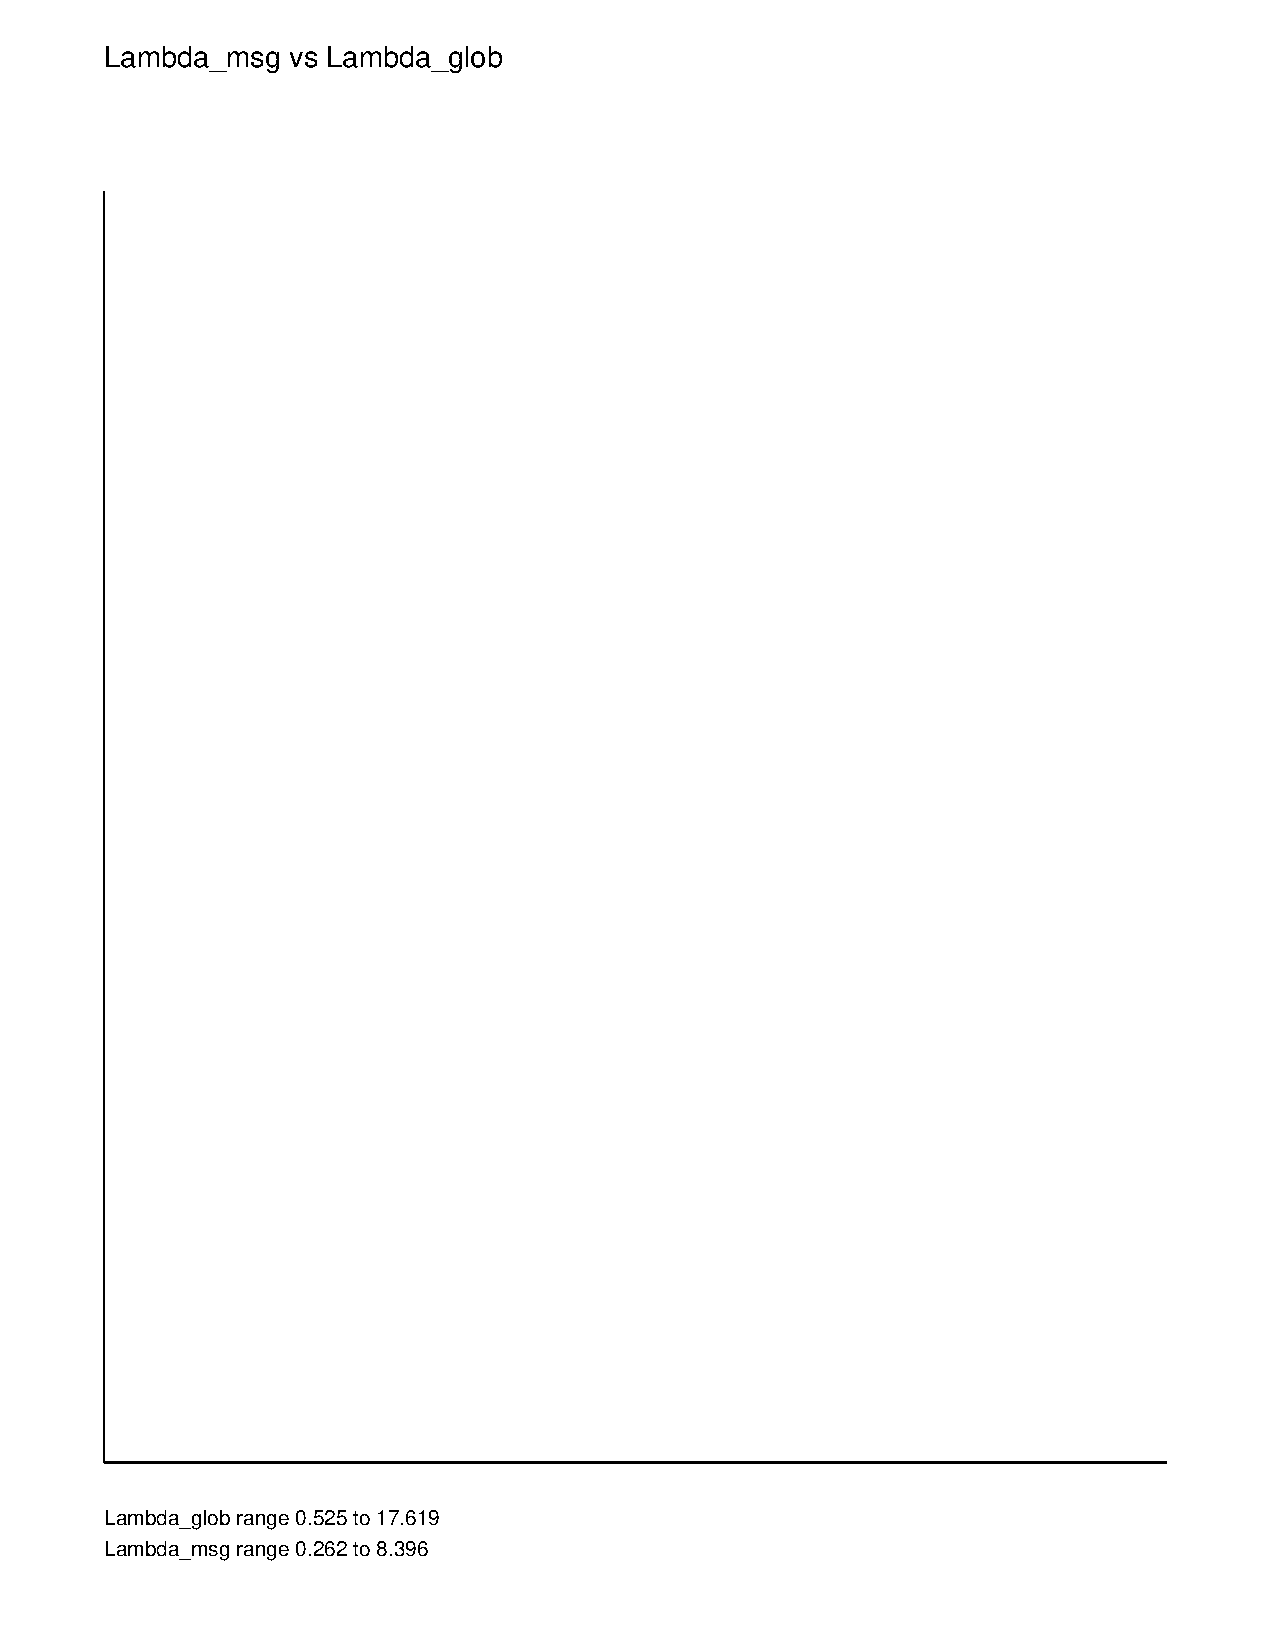
\includegraphics[width=0.46\linewidth]{figures/exp_lambda_msg_vs_lambda_glob.pdf}
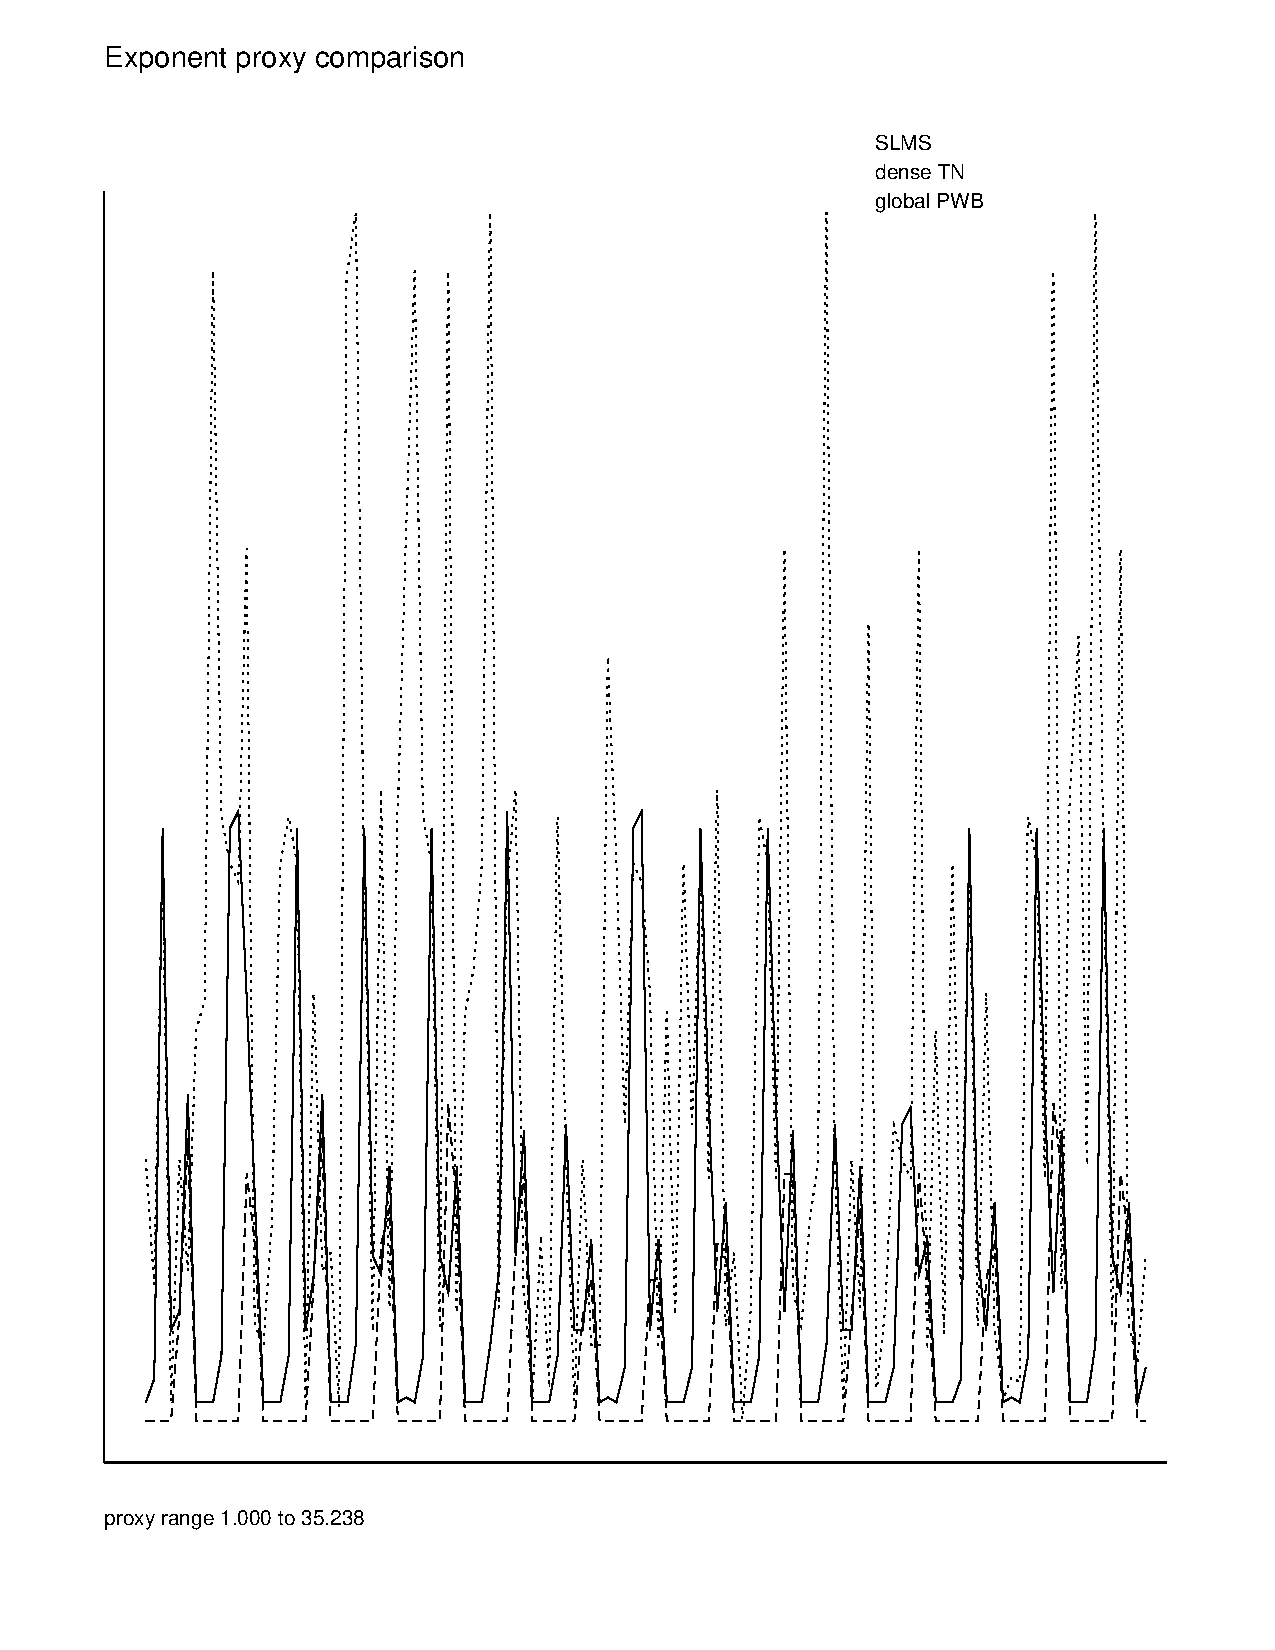
\includegraphics[width=0.46\linewidth]{figures/exp_exponent_proxy_comparison.pdf}
\caption{Fallback certificate-evidence diagnostics. Left: \(\Lammsg\) versus \(\Lambda_{\mathrm{glob}}\). Right: exponent proxy comparison across the generated structured instances. These plots are generated artifacts, but they are not runtime measurements and not parser-generated lambeq data.}
\label{fig:certificate-evidence}
\end{figure}

\begin{figure}[t]
\centering
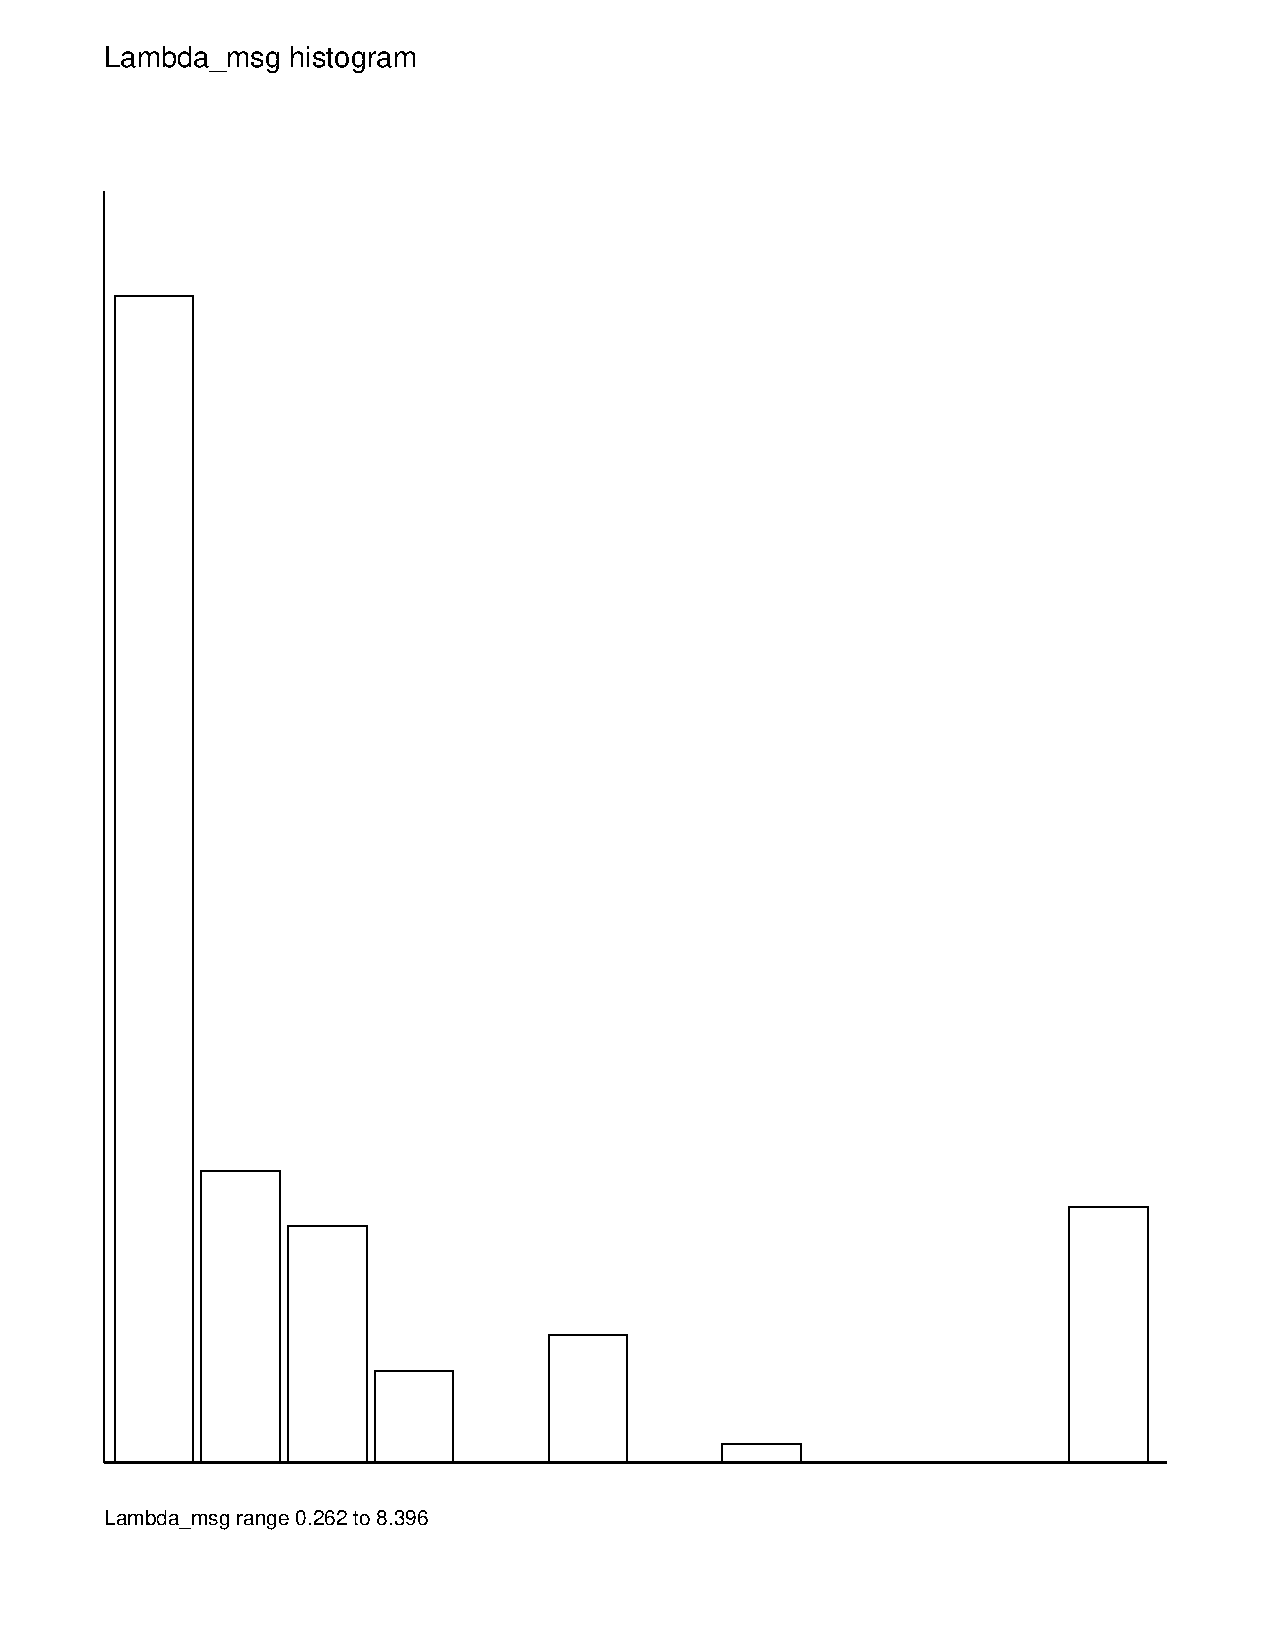
\includegraphics[width=0.46\linewidth]{figures/exp_lambda_msg_histogram.pdf}
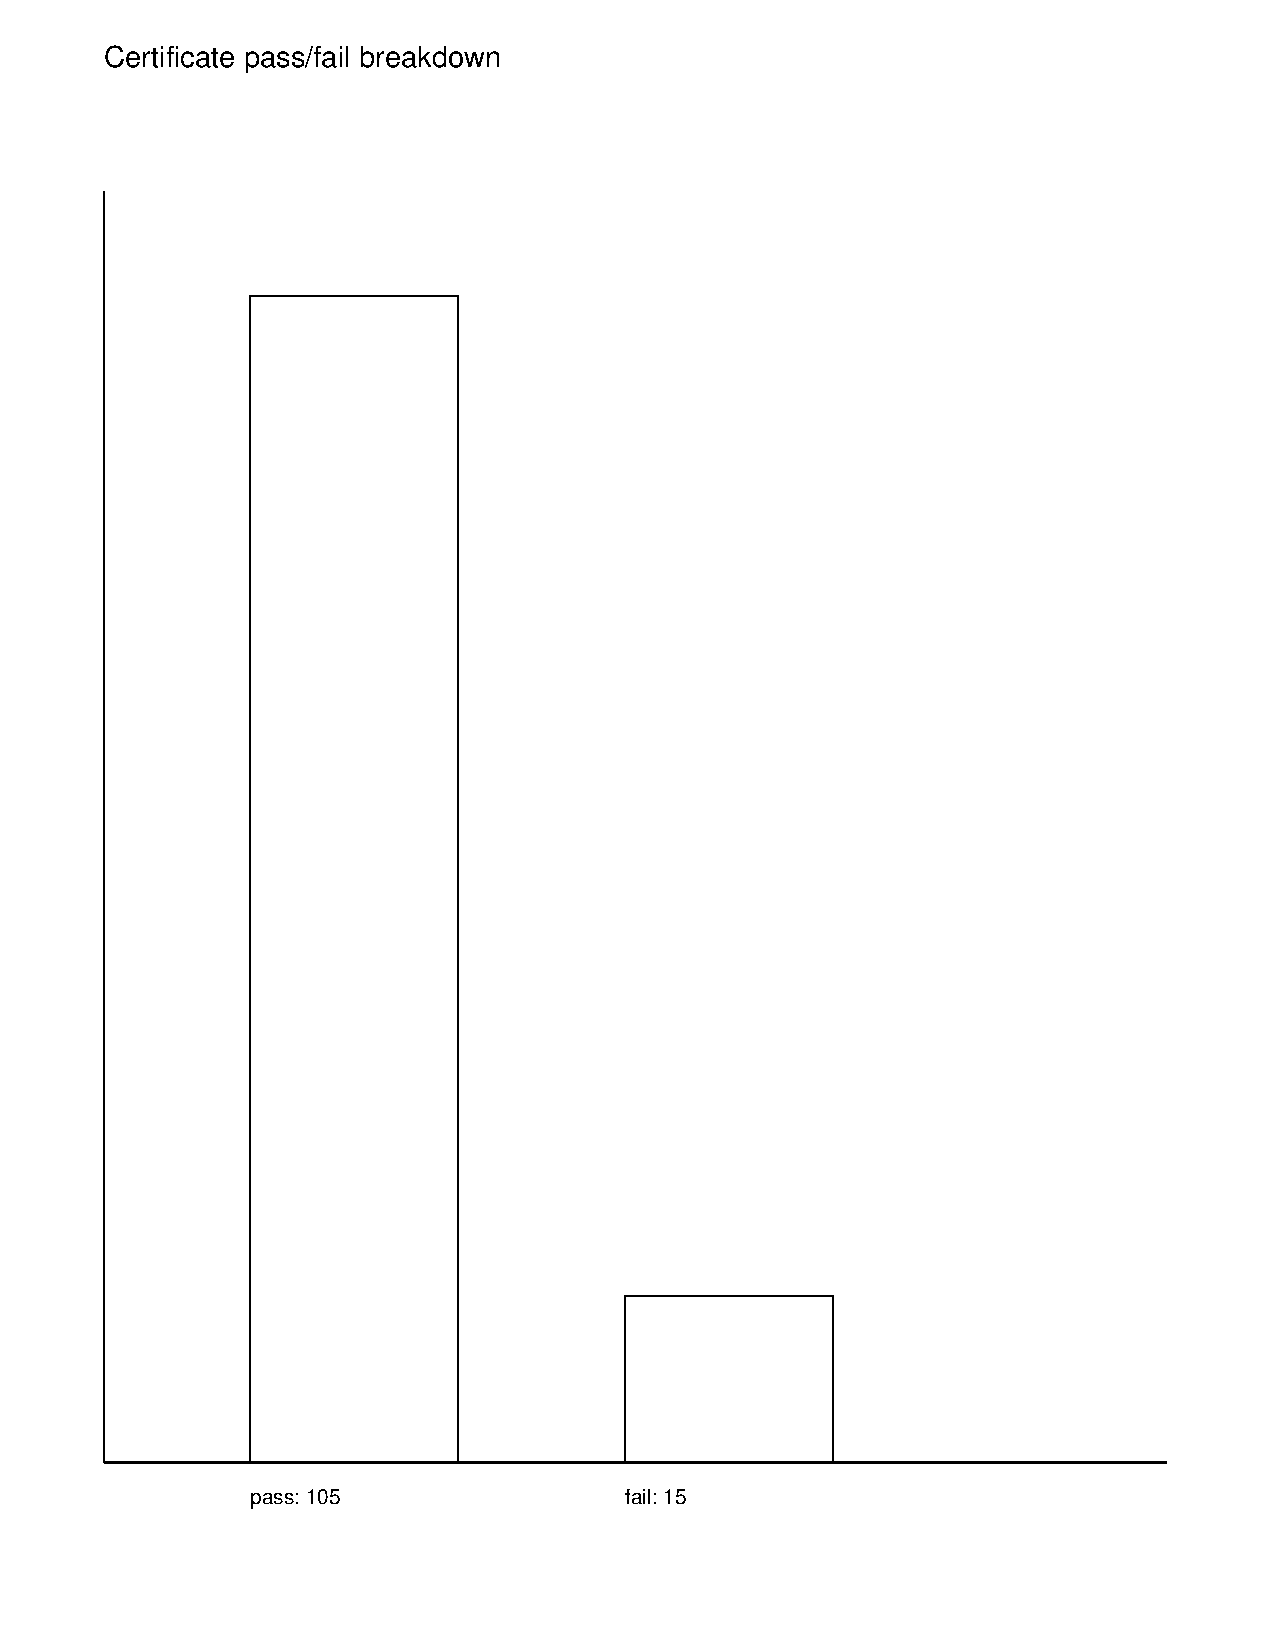
\includegraphics[width=0.46\linewidth]{figures/exp_certificate_pass_rate.pdf}
\caption{Fallback certificate distribution and pass/fail counts. The failure count is intentional: the fallback generator includes negative controls where local marginalization certificates are missing.}
\label{fig:certificate-pass}
\end{figure}

\subsection{Comparison baselines: focused width, ZX, and STN-style upper bounds}
\label{sec:bench-comparators}

The artifact's \texttt{baselines.py} now computes per-instance numerical exponents for three additional comparators. None of them is claimed to dominate SLMS; the purpose is to give an honest empirical reading of where the SLMS exponent sits relative to recent literature.

\paragraph{Codsi--Laakkonen focused tree-width and focused rank-width.}
Implemented exactly via balanced-separator enumeration for instances with \(\le 22\) vertices, with a heuristic upper bound otherwise. Focused rank-width is computed by recursive bipartition of the special set \(S\) (the set of resource bags) with cut-rank evaluated over \(\mathbb F_2\); this is exact for small special sets and an upper-bound diagnostic otherwise. We report the natural-log Codsi--Laakkonen runtime exponent \((\log_{3/2} 4)\cdot\mathrm{frw}_S\cdot\log|S|\) per Theorem~8 of Codsi and Laakkonen~\citep{CodsiLaakkonen2026}, using the implemented focused-rank-width value. Across the 120 fallback instances: median focused tree-width diagnostic is \(4\) (range \(1\)--\(63\)); median focused rank-width diagnostic is \(3\) (range \(1\)--\(25\)); median Codsi--Laakkonen exponent diagnostic is \(37.92\) (range \(2.37\)--\(347.44\)).

\paragraph{ZX-inspired diagnostic (pyzx \texttt{full\_reduce} + Bravyi--Gosset stabilizer rank).}
For each instance we build a synthetic Clifford+\(T\) circuit on \(|V|\) qubits in which a \(T\) gate is placed on the qubit at every resource bag and a \(CZ\) is placed on every parent--child edge (with \(H\) layers at the boundary). We run \(\mathtt{pyzx.simplify.full\_reduce}\) and report \(\alpha_{\mathrm{BG}}\cdot T_{\mathrm{reduced}}\cdot\ln 2\) with \(\alpha_{\mathrm{BG}}=0.396\) \citep{BravyiGosset2016}. This synthetic encoding is consistent across instances but is not the original quantum circuit. Across the 120 fallback instances: median \(T_{\mathrm{reduced}}=16\) (range \(2\)--\(69\)); median ZX exponent is \(4.39\) (range \(0.55\)--\(18.94\)). The artifact also reports a pyzx graph \(k\)-partition heuristic after \(\mathtt{full\_reduce}\), minimizing a conservative partition score \(\max_j \alpha_{\mathrm{BG}}T_j\ln2 + |\partial|\,\ln2+\ln k\) for \(k\le4\). This is a reproducible partition diagnostic, not the Sutcliffe--Kissinger algorithm. \(\mathtt{pyzx.simplify.full\_reduce}\) and this heuristic do not invoke ZX cutting or parametric rewriting; the Sutcliffe--Kissinger \(k\)-partitioning and parametric-rewriting algorithms \citep{Sutcliffe2024KPartition,SutcliffeKissinger2024Cutting,SutcliffeKissinger2025Parametric} are stronger comparators that we do not implement here.

\paragraph{Stabilizer-tensor-network proxy.}
The exact Masot-Llima--Garc\'ia-S\'aez \citep{MasotLlimaGarciaSaez2024} and Nakhl et al.\ \citep{NakhlEtAl2025} algorithms are not implemented in this artifact. We report a tableau-plus-Bravyi--Gosset upper-bound proxy \(\alpha_{\mathrm{BG}}\cdot T+\log\max(1,n_{\mathrm{active\,resource}})\) (natural log) for our synthetic Clifford+\(T\) encoding. Across the 120 instances: median STN-style proxy exponent is \(8.01\) (range \(0.55\)--\(23.30\)). This is not a faithful reimplementation of the published algorithms and not a lower bound on stabilizer-tensor-network simulation; it is an upper-bound comparator only.

\paragraph{Empirical SLMS comparison.}
For each fallback instance, the SLMS exponent \(\weff+2\Lammsg\) (median \(3.57\), range \(1.52\)--\(18.27\)) is compared against the implemented diagnostics on the same instance. Counts where the SLMS exponent is strictly smaller than the comparator diagnostic are: \(101/120\) versus the implemented Codsi--Laakkonen Theorem 8 exponent diagnostic; \(66/120\) versus the pyzx \texttt{full\_reduce}+Bravyi--Gosset diagnostic; \(66/120\) versus the pyzx \(k\)-partition heuristic; and \(69/120\) versus the STN-style upper-bound proxy. These ratios are exponent-bound comparisons on a fixed synthetic encoding and a single fallback corpus; they are not wall-clock simulator comparisons or proofs of separation. A small SLMS exponent on a particular instance is evidence that this certificate identifies an easy regime, not evidence that competing simulators fail.

\paragraph{Wall-clock timings.}
The artifact records per-instance wall-clock seconds for each new comparator. Median wall-clock cost across the 120 instances: focused tree-width and focused rank-width together \(0.12\,\mathrm{s}\) (max \(0.91\,\mathrm{s}\)), pyzx \texttt{full\_reduce} \(5.8\times 10^{-3}\,\mathrm{s}\) (max \(0.04\,\mathrm{s}\)), pyzx partition heuristic \(7.9\times10^{-3}\,\mathrm{s}\) (max \(0.05\,\mathrm{s}\)), and STN-style proxy \(<10^{-4}\,\mathrm{s}\). The lambeq LinearReader sidecar instances also receive these computations but produce zeros because the reader output carries no non-Clifford resource annotations. Figure~\ref{fig:focused-proxy} compares the legacy focused-width proxy against the SLMS exponent.

\subsection{Executed dense contraction and scalar-estimator microbenchmarks}

To separate proxy accounting from executed code, the artifact also runs two small implementation checks. First, \texttt{dense\_contraction\_baseline.py} builds numeric bond-dimension-2 tensor networks from small graph instances and contracts them with \texttt{opt\_einsum}. This is a real dense contraction baseline for generated tensor data, but only on small graph-derived instances; it is not a real lambeq circuit benchmark. In the current run, 24 fallback-derived instances were contracted. The median optimized FLOP estimate was \(212\), the median largest intermediate size was \(8\), and the median contraction time was approximately \(2.2\times 10^{-4}\) seconds. The largest optimized FLOP estimate in this small run was \(176256\), with largest intermediate size \(4096\). A second sidecar dense contraction run on 24 lambeq LinearReader graphs had median optimized FLOP estimate \(124\), median largest intermediate size \(4\), and median contraction time approximately \(1.7\times 10^{-4}\) seconds.

Second, the scalar-estimator script runs a certificate-controlled signed-sampling microbenchmark on 32 passing fallback certificates, with 20000 samples per instance. This tests the sampling dependence and records empirical variance and runtime, but it is not a QNLP simulator. The median absolute error from the synthetic target value \(1\) was \(5.02\times 10^{-3}\), and the median standard error was \(6.66\times 10^{-3}\). These values are reported in the scalar-estimator CSV under \texttt{results/}.

\begin{figure}[t]
\centering
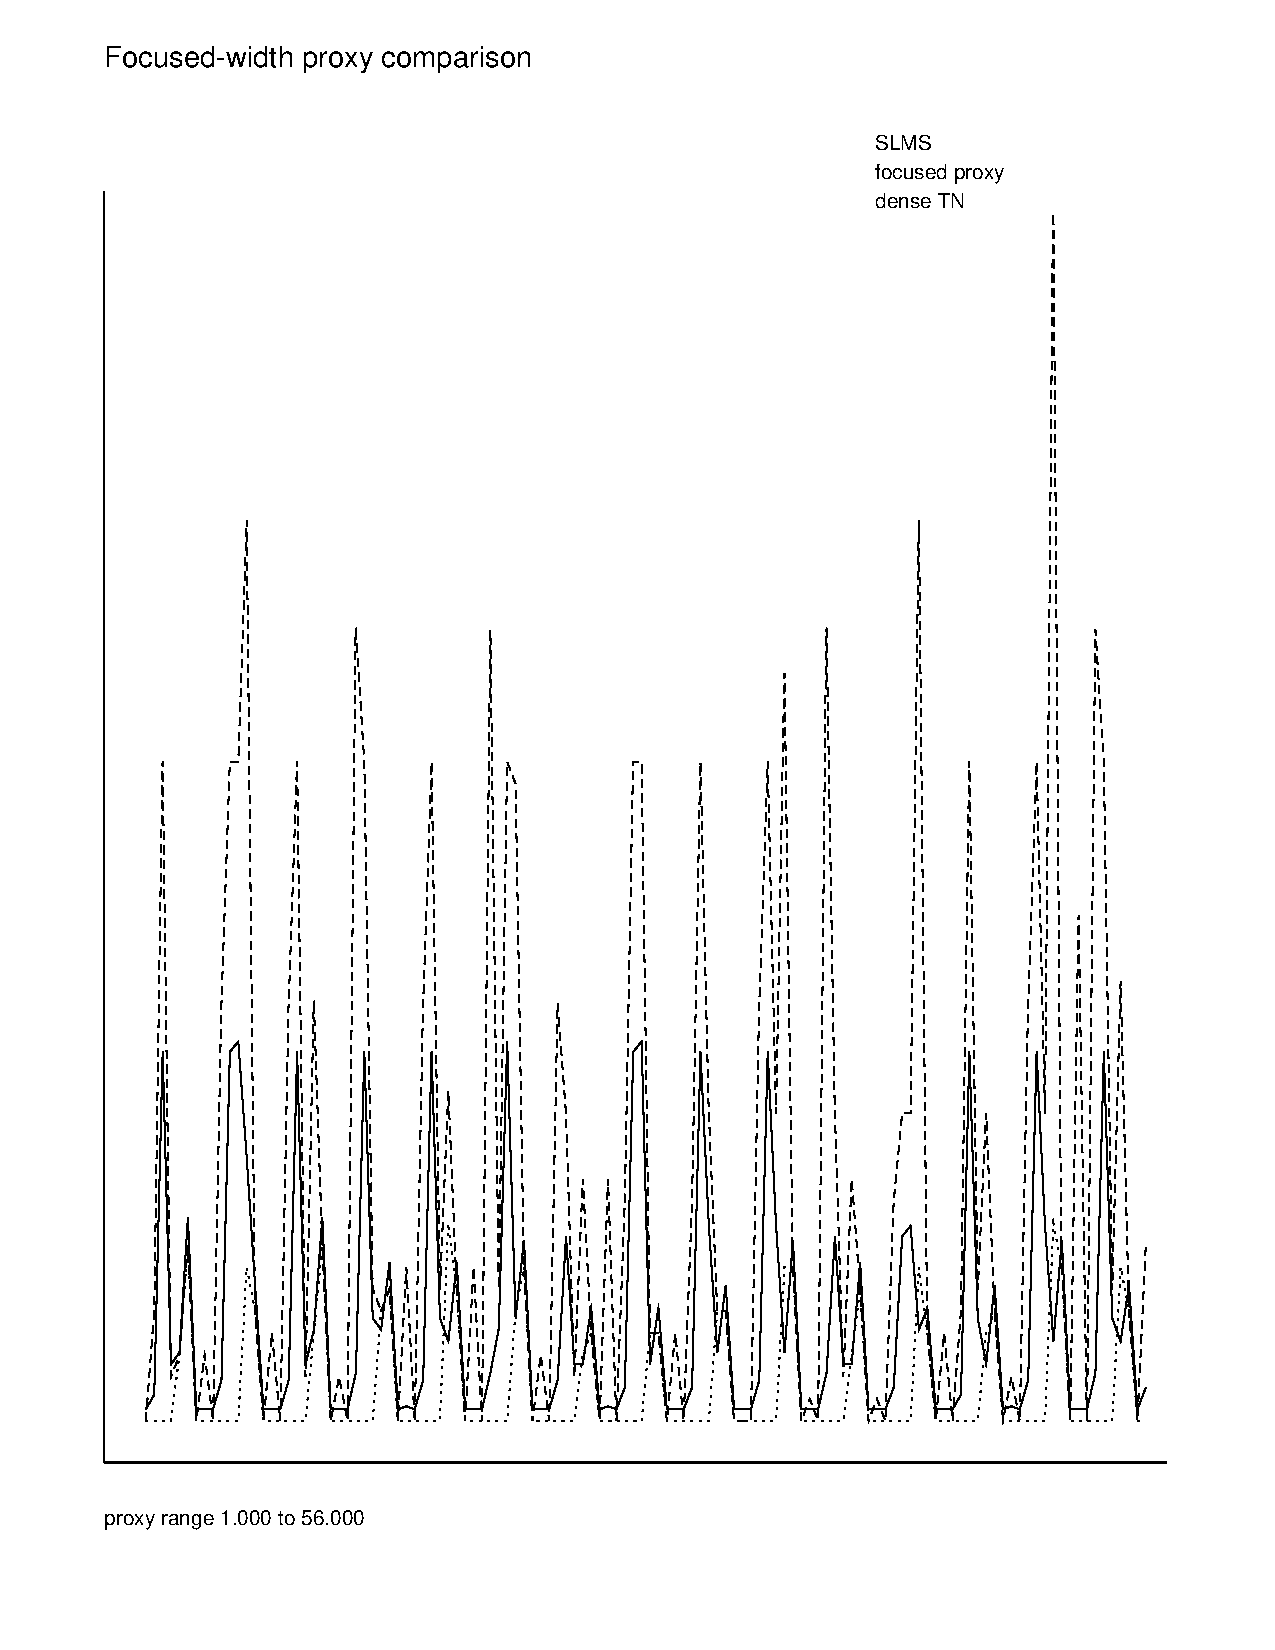
\includegraphics[width=0.48\linewidth]{figures/exp_focused_width_proxy_comparison.pdf}
\caption{Comparison with the implemented focused-width proxy. The plotted quantity is a resource-weighted separator proxy, not exact focused tree-width or focused rank-width.}
\label{fig:focused-proxy}
\end{figure}

\subsection{Circuit-level benchmark families}

\paragraph{Synthetic grammar trees.}
Generate binary and mildly nonbinary parse trees with \(n\) leaves. Assign stabilizer tensors to grammatical reductions and place resource tensors according to controlled modes. This family isolates how \(\Lammsg\) changes under fixed tree shape and active-child declarations.

\paragraph{Synthetic discourse graphs.}
Generate graphs by connecting sentence trees through discourse edges with tunable separator width. Parameters include the number of sentences, average discourse degree, entity coreference edges, and the placement of non-Clifford discourse-update tensors. These graphs test when local marginalizability fails.

\paragraph{lambeq-generated sentence circuits.}
Use lambeq to parse sentences, rewrite diagrams, and instantiate standard ans\"atze. Extract contraction graphs before and after simplification. Compare resource placement under different ansatz choices, including Clifford-only controls and non-Clifford parameterized rotations.

\paragraph{Legal-text-derived composition graphs.}
Use legal corpora such as ILDC or IndianBailJudgments only as possible empirical stress tests for graph structure. The benchmark object is a composition graph extracted from long documents, not a claim about legal AI deployment. The goal is to test whether long, structured documents produce separator and active-child profiles distinct from short sentence datasets.

\subsection{Metrics}

Each full benchmark instance records:
\begin{itemize}[leftmargin=1.2cm]
\item number of tensors or gates;
\item number of qubits, wires, and contracted indices;
\item dense width \(\wTN\) and effective width \(\weff\);
\item number and type of non-Clifford tensors;
\item local costs \(\xi_b\);
\item global burden \(\Lambda_{\mathrm{glob}}\);
\item message burden \(\Lammsg(C,\T)\);
\item active-child profile \(|\Act(b)|\) across bags;
\item \(M_2\), linear stabilizer entropy, or related stabilizer R\'enyi diagnostics for small local states where computable;
\item predicted runtime under pure tensor-network contraction, global-magic simulation, naive hybrid simulation, and SLMS;
\item actual runtime when a simulator implementation is supplied.
\end{itemize}

\subsection{Expected diagnostics}

The current accounting implementation already produces two plots. A full circuit backend would add:
\begin{itemize}[leftmargin=1.2cm]
\item predicted runtime versus \(\wTN\);
\item predicted runtime versus \(\weff\);
\item predicted runtime versus global burden;
\item predicted runtime versus \(\Lammsg\);
\item global burden versus \(\Lammsg\) under clustered and distributed resource placement;
\item phase diagram in \((\weff,\Lammsg)\);
\item active-child heat maps showing which bags dominate message cost.
\end{itemize}

\subsection{Required empirical validation}

The current repository contains synthetic accounting diagnostics, fallback structured certificate evidence, lambeq LinearReader graph-only sidecar evidence, and comparator diagnostics. A submission claiming broad empirical competitiveness would still need, at minimum, the following validation layer:
\begin{itemize}[leftmargin=1.2cm]
\item real lambeq or QDisCoCirc extracted circuits, including the original diagrams, ansatz choices, and simplification passes;
\item dense tensor-network baselines using a standard contraction package and recorded contraction orders;
\item global quasiprobability or stabilizer-decomposition baselines using the same local resource dictionary;
\item focused tree-width, focused rank-width, or low-rank-width ZX-inspired baselines when implementation access permits;
\item ZX cutting or \(k\)-partitioning baselines for Clifford+\(T\)-like diagrams where PyZX/QuiZX-style workflows apply;
\item stabilizer tensor-network baselines, including magic-state-injection variants where available;
\item full certificate output for each instance: \(\T\), \(\wTN\), \(\wTNopt\) or an upper/lower-bound proxy, \(\weff\), every \(\xi_b\), every \(\kappa_b\), all active-child sets \(\Act(b)\), \(\Lambda_{\mathrm{glob}}\), and \(\Lammsg\);
\item runtime, memory, and estimator variance measurements, separated from the synthetic exponent proxies.
\end{itemize}
Absent this layer, the results in this section are only reproducible bookkeeping for the definitions.

\subsection{Reproducibility}

A minimal implementation separates graph generation, circuit generation, decomposition, resource estimation, active-child certification, and simulation. Tree decompositions and active-child sets are stored explicitly. Resource estimates record whether they are exact, convex-programming bounds, analytic formulas for known magic states, or diagnostics such as stabilizer R\'enyi entropy. Legal-text-derived experiments publish only graph-extraction code and dataset instructions consistent with dataset licenses.

\section{Limitations}
\label{sec:limitations}

\subsection{Restricted theorem}

The main theorem applies only to locally marginalizable resource-decomposition networks. This is a real restriction. A general compositional circuit may have resource tensors whose effects remain coherent across several child branches; then the active-child recurrence may collapse to the global product, or the network may fail the local marginalization condition altogether.

\subsection{Why this does not automatically beat treewidth contraction}

If ordinary dense contraction width is already logarithmic, Markov--Shi-style tensor-network contraction already gives polynomial-time simulation. If \(\weff=\wTN\) and \(\Lammsg>0\), Theorem~\ref{thm:main} is not an asymptotic improvement over ordinary dense tensor-network contraction. SLMS is useful only when at least one of the following holds:
\begin{itemize}[leftmargin=1.2cm]
\item stabilizer compression gives \(\weff\ll\wTN\);
\item global magic is high but the message burden is low;
\item resource tensors are modular and locally marginalizable;
\item the benchmark goal is to diagnose where non-stabilizer resource sits relative to separators, not to outperform every contraction method.
\end{itemize}

The stabilizer-grid separation in Proposition~\ref{thm:dense-width-separation} is a separation from dense treewidth parameters. It is not a lower bound against every classical algorithm, since a stabilizer-aware simulator can also exploit the graph-state core. This distinction is important: the paper compares simulation parameters and certified algorithms, not computational complexity lower bounds.

\subsection{Why this does not automatically beat focused-width, ZX, or STN methods}

SLMS is not claimed to supersede recent focused tree-width, focused rank-width, low-rank-width ZX, ZX partitioning, or stabilizer tensor-network simulators \citep{CodsiLaakkonen2026,KuyanovKissinger2026,Sutcliffe2024KPartition,SutcliffeKissinger2024Cutting,SutcliffeKissinger2025Parametric,MasotLlimaGarciaSaez2024,NakhlEtAl2025}. Those methods can exploit graph rewrites, rank-width, stabilizer decompositions, tensor-network partitioning, or stabilizer-state tensor bases in ways that are not captured by \(\weff\) and \(\Lammsg\).

Consequently, a small SLMS certificate is evidence of an easy regime, but a large SLMS burden is not evidence that competing simulators fail. Conversely, the dense-grid example separates SLMS from dense treewidth bounds only; focused-width or stabilizer-aware methods may also simulate it efficiently. A strict separation from these modern competitors would require proving a family with low \(\weff+2\Lammsg\) and provably large focused width, rank width after ZX simplification, partitioning cost, and stabilizer tensor-network cost. No such separation is proved here.

\subsection{Computing the certificates}

The theorem assumes a rooted decomposition, an effective-boundary certificate, local quasiprobability costs, and active-child sets. Computing optimal versions of these objects may be hard. In particular, stabilizer extent, robustness, and related quantities may require nontrivial optimization outside special cases. Benchmarks may need certified upper bounds or proxies rather than exact costs.

\subsection{Artifact and evidence limitations}

The executed artifact run in this repository is not parser-level QNLP evidence. A clean Python 3.11 lambeq installation was created and lambeq imported, but no CCG-grammatical parser path in lambeq 0.5.0 produced parsed diagrams in this environment. \texttt{BobcatParser} failed while retrieving its model from a hardcoded model URL; \texttt{DepCCGParser} could not run because the external \texttt{depccg} package did not build/install in the audited environment; and \texttt{WebParser} failed against the lambeq web service. The exact command outputs are recorded in the artifact logs and blocker reports. The fallback path through lambeq's \texttt{cups\_reader} produces 120 LinearReader graph-only diagrams; these are real lambeq output but not CCG-parsed and carry no non-Clifford resource annotations. The QDisCoCirc probe also found no importable \texttt{qdiscocirc} or \texttt{qdisco\_circ} package in the verified environment.

The 120 fallback structured instances are useful for testing the certificate recurrence, negative controls, output formats, plots, dense microbenchmarks, scalar-estimator microbenchmarks, focused-width and ZX and STN-style comparator computations, and the wall-clock timings reported in Section~\ref{sec:bench-comparators}. They do not prove coverage of real parser-generated lambeq or QDisCoCirc workloads.

The Codsi--Laakkonen focused tree-width and focused rank-width are computed exactly only for instances with \(\le 22\) vertices (focused tree-width) or \(|S|\le 4\) special vertices (focused rank-width); larger instances receive an honest upper bound via greedy elimination or recursive bipartition. The reported Codsi--Laakkonen runtime exponent uses our \(\mathrm{frw}\) upper bound; a smaller true \(\mathrm{frw}\) would shift the comparator. The ZX-inspired diagnostic uses \(\mathtt{pyzx.simplify.full\_reduce}\) and the artifact now adds a simple pyzx \(k\)-partition heuristic, but neither implements Sutcliffe--Kissinger cutting or parametric rewriting. The stabilizer-tensor-network row is a tableau plus Bravyi--Gosset stabilizer-rank \emph{upper bound}; the actual algorithms of Masot-Llima--Garc\'ia-S\'aez \citep{MasotLlimaGarciaSaez2024} and Nakhl et al.\ \citep{NakhlEtAl2025} are not implemented in this artifact. The artifact's small dense-contraction and scalar-estimator microbenchmarks are real wall-clock timings on graph-derived data, but the end-to-end real-QNLP SLMS wall-clock gate reports blocked because no parser-generated resource instances are available.

\subsection{When SLMS is not useful}

SLMS may provide little or no benefit when:
\begin{itemize}[leftmargin=1.2cm]
\item \(\weff\) is close to the ordinary dense width \(\wTN\);
\item \(\Lammsg\) is close to the global burden \(\Lambda_{\mathrm{glob}}\);
\item local marginalization fails and most children must be declared active;
\item continuous trainable rotations occur densely across high-level separators;
\item a focused tree-width, focused rank-width, low-rank-width ZX, ZX-cutting, or stabilizer tensor-network method gives a tighter certificate;
\item ZX simplification removes the non-Clifford structure that SLMS would otherwise charge for;
\item certificate search is as hard as the contraction problem being certified;
\item the task requires multiplicative accuracy or rare-event sampling rather than additive scalar probability estimation.
\end{itemize}

The failure of the SLMS certificate is not evidence of quantum hardness. It only means that this sufficient condition did not certify an easy regime.

\subsection{Diagnostics versus operational overhead}

Stabilizer R\'enyi entropy is not used as an operational runtime parameter. It can be an informative diagnostic, but substituting it for quasiprobability norm or robustness requires a proved inequality for the relevant tensor class.

\subsection{No hardness dichotomy}

Large \(\weff+2\Lammsg\) suggests that this specific simulator may be expensive; it does not prove classical hardness. Conversely, QDisCoCirc conditional hardness results do not automatically imply lower bounds on \(\weff\), \(\Lammsg\), or local marginalizability.

\subsection{Idealized model}

The model abstracts away compilation and hardware noise. This is intentional. The paper studies exact or controlled-error classical simulation of idealized structured circuits, not experimental performance or application utility.

\section{Conclusion}
\label{sec:conclusion}

Structured quantum tensor networks invite a simulation analysis that uses both graph structure and stabilizer resource theory. Treewidth bounds capture separators but ignore whether the tensors crossing them are free or resourceful. Global magic bounds capture non-stabilizer content but ignore where that content sits in a compositional graph.

The contribution is a certificate-based separator-local theorem for locally marginalizable resource-decomposition networks. The key parameter is \(\Lammsg\), computed by an explicit active-child recurrence, together with the stabilizer-compressed width \(\weff\). The scalar sampling dependence is \(\exp(2\Lammsg)\). This theorem proves a restricted easy regime and gives pedagogical separations from naive global-magic accounting on constant-boundary families with many locally consumed resources, including a path-active variant where unresolved resource randomness persists through \(O(\log n)\) separators rather than vanishing immediately at leaves. It also gives a stabilizer-grid parameter separation between dense treewidth bounds and stabilizer-compressed separator-local certificates.

The accompanying artifact makes the certificate concrete. It attempts real lambeq extraction when available, falls back to explicitly labelled structured instances otherwise, exports \(\xi_b\), \(\kappa_b\), \(\Act(b)\), \(\Lammsg\), \(\Lambda_{\mathrm{glob}}\), width proxies, and comparator exponent proxies, and records the run manifest. In the executed run reported here, lambeq imported successfully in a Python 3.11 environment, but no Bobcat/DepCCG/CCG parser produced parsed diagrams for the sample corpus. A local lambeq LinearReader path did produce 120 graph-only diagrams with no resource annotations, and the run therefore used 120 fallback structured instances as the primary nontrivial certificate evidence, with 105 certificate passes and 15 deliberate certificate failures. The artifact also includes small dense-contraction and scalar-estimator microbenchmarks on graph-derived data. The generated plots and CSV files are certificate-evidence diagnostics rather than empirical parser-level QNLP results.

SLMS should be viewed as a sufficient-condition framework for identifying classically easy structured quantum tensor networks. Its value is diagnostic: it makes explicit when local non-stabilizer resources are consumed before loading high-level separators, and records this in a reproducible certificate. The present artifact demonstrates the mechanics of the certificate, its failure modes, and its comparison to several implemented proxy diagnostics. Extending the same workflow to parser-generated QNLP/QDisCoCirc resource instances and to exact ZX/STN implementations remains future work.


\section*{Declarations}

\paragraph*{Funding.} This work received no external funding.

\paragraph*{Competing interests.} The authors declare no competing interests.

\paragraph*{Code and data availability.} The source code, experiment scripts, generated CSV files, plots, environment logs, parser-failure logs, and worked-certificate data are archived at [Zenodo DOI to be inserted after release] and mirrored at [GitHub URL to be inserted after release]. The repository also contains a hard-blocker ledger distinguishing exact unavailable baselines from implemented proxy diagnostics.

\appendix
\section{Tree Decompositions and Separator Accounting}
\label{app:tree}

This appendix records conventions used in the main text. Let \(G=(V,E)\) be the contraction graph of the scalar network used for \(p_C(x)\). A tree decomposition \((T,\beta)\) is normally defined on vertices of \(G\), but tensor contraction cost is determined by open indices. For a bag \(b\), let \(I_b\) be the set of tensor indices incident to tensors in \(\beta(b)\) that are not fully contracted inside the portion of the elimination represented by \(b\). A dense message on \(I_b\) has dimension \(\prod_{i\in I_b}d_i\).

For bounded-degree qubit networks, vertex width and index width differ by at most constant factors. For language diagrams, however, reductions and word tensors may have nonuniform arity. It is therefore safer to state algorithmic costs in terms of
\[
w=\max_{e\in E(T)}\sum_{i\in S_e}\log_2 d_i,
\]
where \(S_e\) is the separator index set for the message crossing \(e\).

\subsection{Rooted message convention}

Root \(T\) at \(r\). For an edge \(e=(b\to c)\), remove \(e\) and let \(T_c\) be the component containing \(c\). The message \(m_{c\to b}\) is a tensor on \(S_e\) obtained by contracting all tensors assigned to bags in \(T_c\) and summing all internal indices in that component. The root scalar is obtained by contracting the messages incident to \(r\) with tensors assigned to \(r\).

\subsection{Nice decompositions}

For implementation, it is convenient to convert \((T,\beta)\) to a nice tree decomposition with introduce, forget, join, and leaf bags. This conversion increases the number of bags polynomially and does not increase dense width. The message burden must be transported carefully: introducing auxiliary bags with \(\xi_b=1\), \(\kappa_b=1\), and no active children leaves \(\Lammsg\) unchanged, while splitting a bag with resource tensors requires either keeping the joint assignment at one bag or proving that the split preserves the local expansion and active-child certificates.

\subsection{Hypergraphs}

If a tensor index connects more than two tensors, the contraction structure is a hypergraph. Two standard reductions are possible. One may use a hypertree decomposition directly, or introduce equality/copy tensors to obtain an ordinary graph. The latter can change stabilizer structure: copy tensors in the computational basis are stabilizer tensors, but copy tensors in arbitrary bases need not be free. The main text assumes either ordinary graphs or a hypergraph reduction that preserves the declared free/resource partition.

\section{Stabilizer and Quasiprobability Decompositions}
\label{app:stabilizer}

This appendix relates common magic measures to the primary local cost \(\xi(A)\). In the theorem, \(\xi(A)\) means a certified free-tensor quasiprobability \(\ell_1\) cost. Other measures are used only insofar as they provide decompositions or upper bounds.

\subsection{Stabilizer rank and extent}

For a pure \(n\)-qubit state \(\ket{\psi}\), the stabilizer rank \(\chi(\psi)\) is the minimum number of stabilizer states needed in an exact linear decomposition
\[
\ket{\psi}=\sum_{j=1}^{\chi} c_j\ket{\phi_j}.
\]
Approximate stabilizer rank permits approximation in norm or fidelity and is used in simulation algorithms where small state error induces controlled output error. Stabilizer extent is the squared minimum \(\ell_1\)-norm of stabilizer decompositions in common conventions:
\[
\xi_{\mathrm{ext}}(\psi)
=\min_{\psi=\sum_j c_j\phi_j}\left(\sum_j |c_j|\right)^2.
\]
Because conventions differ by squares, the main text uses a generic \(\xi(A)\) and places squares explicitly in variance statements.

\subsection{Robustness of magic}

Robustness of magic expresses a state or operation as a signed combination of free stabilizer objects and minimizes the \(\ell_1\) weight. It has an operational role in quasiprobability simulation and magic-state resource theory. For mixed states,
\[
\rho=\sum_j q_j\sigma_j,\qquad \sigma_j\in\Sstab,
\]
with real coefficients \(q_j\), the relevant cost is typically \(\sum_j |q_j|\), minimized over stabilizer decompositions. Channel robustness and related quantities can be defined analogously through free channels or Choi states, with care about normalization.

\subsection{Dyadic negativity and quasiprobability norm}

Quasiprobability simulation chooses a representation in which free operations are efficiently sampleable and resource operations have signed representations. The cost is an \(\ell_1\) norm of the signed representation. Dyadic negativity is one such measure adapted to stabilizer operations over qubits. The SLMS theorem is compatible with any such measure satisfying:
\begin{enumerate}[leftmargin=1.2cm]
\item exact reconstruction of the resource tensor as a signed combination of free tensors;
\item efficient sampling from absolute weights;
\item a second-moment bound controlled by the square of the \(\ell_1\) norm;
\item closure of sampled free tensors under the message-passing contraction.
\end{enumerate}

\subsection{Worked examples for \texorpdfstring{\(\kappa_b\)}{kappa}}
\label{app:kappa-example}

The factor \(\kappa_b\) is a certified local expansion factor for the coefficient map induced by contracting a bag. Fix a finite free dictionary \(\{F_i\}_{i=1}^m\) for the incoming representatives and \(\{G_j\}_{j=1}^{m'}\) for the outgoing representatives. If the local contraction sends
\[
F_i\longmapsto \sum_j (L_b)_{j i}G_j,
\]
then a coefficient vector \(q\) is mapped to \(L_b q\). A sufficient bound on the outgoing \(\ell_1\) cost is
\[
\norm{L_b q}_1\le \norm{L_b}_{1\to 1}\norm{q}_1,
\qquad
\kappa_b=\norm{L_b}_{1\to1}
=\max_i\sum_j |(L_b)_{j i}|.
\]
The message recurrence is therefore
\[
\Gamma_b=\kappa_b\xi_b\prod_{c\in\Act(b)}\Gamma_c .
\]

For a stochastic classical marginalization map, let \(G_0,G_1\) be the two outgoing classical basis messages and suppose the local map is
\[
L_{\mathrm{stoch}}
=
\begin{pmatrix}
1 & 0 \\
0 & 1
\end{pmatrix}
\quad\text{or more generally}\quad
L_{j i}\ge 0,\quad \sum_j L_{j i}\le 1 .
\]
Then \(\norm{L_{\mathrm{stoch}}}_{1\to1}\le 1\), so \(\kappa_b=1\). This is the case for normalized classical postprocessing, erasure, and marginalization maps used in the leaf-local examples.

As a nontrivial expansion example, consider changing from a one-dimensional signed representative \(F_+\) to a two-element outgoing dictionary by
\[
F_+\longmapsto G_0-G_1 .
\]
The coefficient matrix is a single column \(L=(1,-1)^T\), hence
\[
\kappa_b=\norm{L}_{1\to1}=|1|+|-1|=2 .
\]
A bag using this map doubles the certified coefficient norm, and the factor is explicitly charged in \(\Gamma_b\). Thus \(\kappa_b\) is not a hidden assumption: it is a local certificate that must be computed, upper-bounded, or conservatively absorbed by marking a larger region active.

\subsection{Operational measure used in the theorem}

The primary operational measure is the generic free-tensor quasiprobability \(\ell_1\) norm. Stabilizer extent, robustness, and dyadic negativity are treated as instantiations or upper bounds, not as separate theorem-level primitives. Comparing the resulting \(\Lammsg\) certificates under several decomposition families is a separate empirical and algorithmic task.

\section{Variance Bounds}
\label{app:variance}

This appendix expands the variance calculation used in Lemma~\ref{lem:message-recurrence} and Theorem~\ref{thm:main}. Suppose a scalar tensor contraction can be written as
\[
p=\sum_{\omega} q(\omega) z(\omega)
\]
where \(q\) is a signed or complex quasiprobability representation. Let
\[
\gamma=\sum_{\omega}|q(\omega)|.
\]
Sampling \(\omega\) from \(Q(\omega)=|q(\omega)|/\gamma\) and returning
\[
Z=\gamma\,\operatorname{phase}(q(\omega))\,z(\omega)
\]
gives \(\E[Z]=p\). If \(|z(\omega)|\le B\), then
\[
\E[|Z|^2]\le \gamma^2 B^2.
\]
Thus \(N=O(\gamma^2B^2\eps^{-2})\) samples suffice for constant-probability additive estimation, with logarithmic amplification for failure probability \(\delta\).

In global quasiprobability simulation, \(\gamma\) is the product of all local \(\ell_1\) costs. In SLMS, Lemma~\ref{lem:message-recurrence} proves for locally marginalizable networks that the effective \(\gamma\) for the hardest message is bounded by
\[
\gamma_{\mathrm{eff}}\le \exp(\Lammsg(C,\T)).
\]
Consequently the sampling term in Theorem~\ref{thm:main} is explicitly \(\exp(2\Lammsg(C,\T))\). The bounded term \(B\) is accounted for by the effective active boundary dimension \(2^{O(\weff)}\) and by normalization conventions for local tensors.

\subsection{Median-of-means}

Let \(Z_1,\ldots,Z_N\) be independent unbiased estimators with variance at most \(\sigma^2\). Partition the samples into \(K=O(\log(1/\delta))\) groups, each of size \(M=O(\sigma^2/\eps^2)\). Compute the mean in each group and return the median. Standard median-of-means analysis gives additive error \(\eps\) with failure probability at most \(\delta\). This avoids requiring bounded support beyond a second-moment bound.

\subsection{Message-table estimators}

The main theorem estimates the root scalar. If an implementation instead estimates intermediate messages as random tensors, it must choose a norm in which to control their second moments and must include the active-boundary table dimension \(D_b\le 2^{O(\weff)}\), per-entry accuracy, and union bounds. The local recurrence in Lemma~\ref{lem:message-recurrence} controls normalized entries or normalized linear functionals through the certified coefficient-norm factors \(\kappa_b\). Replacing these local certificates by a sharper general separator rule is part of the broader separator-factorization conjecture.

\section{QNLP Graph Extraction}
\label{app:qnlp-extraction}

This appendix sketches a reproducible graph-extraction procedure for follow-up experiments.

\subsection{Sentence-level lambeq circuits}

For each sentence:
\begin{enumerate}[leftmargin=1.2cm]
\item parse the sentence with a fixed parser and record parser version and options;
\item build the string diagram and apply a fixed rewrite system;
\item instantiate the ansatz with a declared number of qubits per grammatical type;
\item export the circuit or tensor network;
\item build the contraction graph for the chosen output probability;
\item identify Clifford/stabilizer tensors and resource tensors;
\item compute a tree decomposition and separator profile.
\end{enumerate}

The extraction records both the pre-rewrite and post-rewrite graphs, since rewriting can materially change treewidth and resource placement.

\subsection{Discourse and document graphs}

For discourse-level circuits, the graph includes sentence modules, entity wires, coreference edges, discourse-relation tensors, question tensors, and answer effects. The extraction must distinguish linguistic edges from tensor-contraction edges. Only the latter define \(G_C\), although the former are useful metadata for interpreting separators.

\subsection{Long legal documents as stress tests}

Legal corpora such as ILDC and IndianBailJudgments may be used to create long-document composition graphs with citations, facts, issues, holdings, and paragraph-level relations. In this paper they are benchmark sources only. The graph-extraction task does not encode legal predictions as a claimed application. It measures whether long formal documents produce contraction graphs with distinctive width and separator-local resource profiles.

\section{Additional Examples}
\label{app:examples}

\subsection{Tree with locally consumed non-scalar resources}

Consider a balanced binary tree of depth \(h\) with one resource tensor of cost \(\xi>1\) attached to each leaf module. In Example~\ref{prop:improvement}, each leaf locally consumes a \(\ket{T}\) state by a Pauli measurement and exports a one-bit classical stabilizer boundary message. Parent nodes combine these messages by Clifford XOR maps. The global magic proxy is
\[
\sum_A\log\xi(A)=2^h\log\xi,
\]
while the message burden is \(O(\log\xi)\) because every resource is locally marginalized before reaching its parent. This separates SLMS from naive global sampling. It does not by itself separate SLMS from dense treewidth contraction, since the underlying tree has small dense width.

\subsection{Chain with resources on every edge}

For a chain of \(n\) tensors with resource cost \(\xi\) on each edge interaction, every separator cuts the chain into a prefix and suffix. If the active-child recurrence keeps the child active at every step, then \(\Lammsg\) grows linearly in the chain length, matching the global product up to constants. This example shows that separator-local magic is not automatically smaller than global magic.

\subsection{Clustered discourse resource}

Suppose a document graph consists of \(k\) sentence subtrees connected by a discourse hub tensor. If all non-Clifford tensors are inside sentence subtrees and each sentence subtree is locally marginalized, \(\Lammsg\) may remain small even for large \(k\). If the hub tensor itself is non-Clifford and has high arity, then it loads a high-level separator and may dominate both \(\weff\) and \(\Lammsg\). This distinction is invisible to a global count of non-Clifford gates.

\section{Certification Algorithms for Stabilizer Backends}
\label{app:certification}

This appendix makes the certificate requirements in Section~\ref{sec:certification} more concrete. The algorithms below are sufficient tests, not complete characterizations. If a test fails, the conservative action is to enlarge the active boundary, mark the child active, or record an additional local norm factor \(\kappa_b\). The failure of a certificate is therefore not evidence of hardness.

\subsection{CERTIFY-FREE-REGIONS}

\begin{center}
\fbox{\begin{minipage}{0.93\linewidth}
\textbf{Algorithm CERTIFY-FREE-REGIONS}
\begin{enumerate}[leftmargin=1.0cm]
\item Input a tensor network with tags \(\mathrm{free}\), \(\mathrm{resource}\), or \(\mathrm{unknown}\).
\item Build the induced graph on tensors tagged \(\mathrm{free}\).
\item Compute its connected components.
\item For each component, record boundary legs incident to resource, unknown, output, or active-child tensors.
\item Return the free components and their boundary metadata.
\end{enumerate}
\end{minipage}}
\end{center}

\subsection{COMPUTE-WEFF-UPPER}

For a free subnetwork \(H\) with boundary legs \(B\), a stabilizer backend can represent the induced boundary relation by a tableau or, for classical wires, by an affine relation over \(\mathbb F_2\). A conservative compression procedure is:
\begin{enumerate}[leftmargin=1.2cm]
\item contract the free Clifford, Pauli-measurement, preparation, discard, and classical-copy tensors using a tableau simulator;
\item record the stabilizer constraints on boundary Paulis and the classical affine constraints on computational-basis wires;
\item mark as dense-active every boundary leg incident to an unresolved resource tensor, to a failed tableau update, or to a non-stabilizer effect;
\item count only the remaining dense-active subsystem in \(D_e^{\mathrm{act}}\).
\end{enumerate}
This gives the certified upper bound
\[
\weff\le \max_e \log_2 D_e^{\mathrm{act}}.
\]
If the tableau representation contains measurements with branch-dependent non-Clifford corrections, those branch labels are dense-active unless they are immediately marginalized by an \(\ell_1\)-nonexpansive map.

\begin{center}
\fbox{\begin{minipage}{0.93\linewidth}
\textbf{Algorithm COMPUTE-WEFF-UPPER}
\begin{enumerate}[leftmargin=1.0cm]
\item Input free-region certificates and a rooted tree decomposition.
\item For each separator \(e\), list dense tensor-network boundary legs \(S_e^{\mathrm{TN}}\).
\item Remove legs represented entirely by tableau, affine stabilizer, or normalized classical stochastic data.
\item Count the remaining active dense dimension \(D_e^{\mathrm{act}}\).
\item Return \(\max_e\log_2D_e^{\mathrm{act}}\).
\end{enumerate}
\end{minipage}}
\end{center}

\subsection{Syntactic free-region detection}

Given a labelled tensor network, form the induced subgraph on tensors whose labels are certified free: stabilizer states and effects, Clifford channels, Pauli measurements, computational-basis preparations and discards, classical stochastic maps with nonnegative columns of sum at most one, and previously certified free mixtures. Connected components of this subgraph are candidate free regions. Boundary legs adjacent to resource tensors or active child messages are exported as active legs; all other boundary information is stored in the tableau or affine representation.

This procedure is intentionally syntactic. It does not try to discover hidden Clifford structure inside an arbitrary dense tensor. A stronger implementation can improve the certificate by applying local Clifford simplification, ZX or circuit rewriting, or small-dimensional membership tests before the free-region pass.

\subsection{CERTIFY-ACTIVE-CHILDREN}

Let \(c\) be a child of \(b\). Write \(K_{b,c}\) for the local map obtained by contracting the message boundary of \(c\) with the tensors at \(b\) that consume that boundary, leaving only the outgoing boundary of \(b\) open. A sufficient inactive-child certificate is one of the following.

\paragraph{Finite stabilizer boundary.}
If the certified child message ranges over a finite list \(\mathcal F_c\) of normalized stabilizer representatives on a constant-size boundary, enumerate \(F\in\mathcal F_c\) and check that \(K_{b,c}(F)\) is either a normalized free representative or a deterministic active-boundary table with \(\ell_1\) cost at most one. For qubit boundaries of size \(O(1)\), this can be implemented by tableau membership plus exact arithmetic for the finite coefficient table.

\paragraph{Classical stochastic boundary.}
If the child boundary is classical and \(K_{b,c}\) is represented by a real matrix \(K\), it is enough to verify
\[
K_{ij}\ge 0,\qquad \sum_i K_{ij}\le 1
\]
for every column \(j\). Then \(K\) maps normalized nonnegative child messages to subnormalized nonnegative messages and does not increase the coefficient \(\ell_1\) norm.

\paragraph{Affine stabilizer relation.}
If \(K_{b,c}\) is a Clifford or classical affine relation, verify by symplectic or affine-rank computation that it maps the child stabilizer relation into the outgoing stabilizer relation. Any leftover boundary bit or Pauli frame bit that is not fixed by this relation is counted as active.

These checks are local. They certify \(c\notin\Act(b)\) only for the chosen decomposition and chosen normalization of the local tensors.

\begin{center}
\fbox{\begin{minipage}{0.93\linewidth}
\textbf{Algorithm CERTIFY-ACTIVE-CHILDREN}
\begin{enumerate}[leftmargin=1.0cm]
\item Process the rooted decomposition bottom-up.
\item For each child \(c\) of \(b\), construct the local map \(K_{b,c}\).
\item If one of the finite stabilizer, classical stochastic, or affine stabilizer checks succeeds, set \(c\notin\Act(b)\).
\item Otherwise set \(c\in\Act(b)\).
\item Return all active-child sets.
\end{enumerate}
\end{minipage}}
\end{center}

\subsection{CERTIFY-L1-NONEXPANSIVE}

For active children and local resource expansions, collect the finite coefficient basis used in the proof of Lemma~\ref{lem:message-recurrence}. The local contraction at \(b\) induces a coefficient matrix \(L_b\). A sufficient nonexpansiveness certificate is
\[
\norm{L_b}_{1\to1}=\max_j\sum_i |(L_b)_{ij}|\le 1.
\]
If this norm is \(L_b^\ast>1\), set \(\kappa_b=L_b^\ast\) and use the recurrence \(\Gamma_b=\kappa_b\xi_b\prod_{c\in\Act(b)}\Gamma_c\). This convention is useful in implementations because it avoids treating small normalization mismatches as certificate failures.

\begin{center}
\fbox{\begin{minipage}{0.93\linewidth}
\textbf{Algorithm CERTIFY-L1-NONEXPANSIVE}
\begin{enumerate}[leftmargin=1.0cm]
\item Input a local coefficient map \(L_b\) in the chosen free representative basis.
\item Compute or upper-bound \(\norm{L_b}_{1\to1}=\max_j\sum_i |(L_b)_{ij}|\).
\item If the bound is finite, output \(\kappa_b=\norm{L_b}_{1\to1}\).
\item If no finite certified bound is available in the chosen representation, fail the local certificate and mark the affected messages active or merge bags.
\end{enumerate}
\end{minipage}}
\end{center}

\subsection{Greedy active-child certification}

The following bottom-up rule is the backend version of the active-child recurrence.
\begin{enumerate}[leftmargin=1.2cm]
\item For each leaf, compute or import the local quasiprobability expansion and its cost \(\xi_b\).
\item For an internal bag \(b\), try the inactive-child marginalization test for each child \(c\).
\item If the test succeeds, set \(c\notin\Act(b)\) and pass only the deterministic free or active-boundary message certified by the test.
\item If the test fails, set \(c\in\Act(b)\) and retain the child message expansion in the recurrence.
\item Run CERTIFY-L1-NONEXPANSIVE and record \(\kappa_b\).
\item Set \(\Gamma_b=\kappa_b\xi_b\prod_{c\in\Act(b)}\Gamma_c\).
\end{enumerate}
The greedy rule is not guaranteed to minimize \(\Lammsg\). It is a constructive certificate generator. Optimizing over decompositions, resource assignments, local normalizations, and active-child choices remains an open algorithmic problem.

\subsection{Worked certificate for a two-leaf grammar tree}
\label{app:worked-certificate}

This example records all certificate data for the smallest nontrivial locally marginalizable tree. Let the rooted decomposition have two leaf bags \(b_1,b_2\) and one root bag \(r\). Each leaf contains a lexical resource module consisting of a \(\ket T\)-type resource followed by a Pauli measurement that writes a classical bit to the phrase boundary. The root applies a free XOR map to the two incoming bits and measures whether the output bit is \(0\).

\paragraph{Tree and dense width.}
Use \(T\) with edges \(b_1-r\) and \(b_2-r\). The dense tensor-network separator across either edge carries one classical bit, so \(\wTN=1\) for this decomposition. The same bit is a computational-basis stabilizer message after local marginalization, so the active dense boundary is empty and \(\weff=0\) if the bit is represented symbolically as a free classical message. If an implementation stores the bit as a dense two-entry table, then \(\weff\le 1\); both are valid certificates with different bookkeeping conventions.

\paragraph{Local costs.}
Let the certified free-tensor quasiprobability cost of each \(\ket T\)-module be \(\xi_T>1\). Assign the two resources to \(b_1\) and \(b_2\), giving
\[
\xi_{b_1}=\xi_{b_2}=\xi_T,\qquad \xi_r=1.
\]
The Pauli measurement and the root XOR are free stochastic or Clifford maps. Their coefficient maps are \(\ell_1\)-nonexpansive in the chosen free dictionary, so
\[
\kappa_{b_1}=\kappa_{b_2}=\kappa_r=1.
\]

\paragraph{Active-child sets.}
At each leaf, the resource label is consumed before the message reaches the root. The outgoing leaf message is a normalized free classical mixture. Therefore both children of the root pass the inactive-child check:
\[
\Act(r)=\emptyset.
\]
Leaves have no children.

\paragraph{Message recurrence.}
The recurrence gives
\[
\Gamma_{b_1}=\xi_T,\qquad
\Gamma_{b_2}=\xi_T,\qquad
\Gamma_r=\kappa_r\xi_r=1.
\]
Hence
\[
\Lammsg=\max\{\log\xi_T,\log\xi_T,0\}=\log\xi_T.
\]
The global burden is instead
\[
\Lambda_{\mathrm{glob}}=\log\xi_{b_1}+\log\xi_{b_2}=2\log\xi_T.
\]
For this two-leaf example the difference is only a constant factor. For the balanced \(n\)-leaf family in Example~\ref{prop:improvement}, the same local certificate repeats independently at every leaf and yields \(\Lammsg=\log\xi_T\) while \(\Lambda_{\mathrm{glob}}=n\log\xi_T\).

\paragraph{Scalar estimator.}
The scalar event is the root parity outcome. The SLMS scalar estimator samples the active recurrence. Since the root has no active children and the leaf labels have been locally marginalized, the root scalar can be computed by contracting free classical messages. The variance bound is nevertheless consistent with Theorem~\ref{thm:main}: the sampling factor is at most \(\exp(2\Lammsg)=\xi_T^2\), independent of the number of locally repeated leaves in the balanced extension.

\section{Worked Certificate on a Fallback Lambeq-Compatible Structured Instance}
\label{app:worked-experiment-certificate}

This appendix records one complete certificate produced by the artifact command recorded in \texttt{results/run\_manifest.json}.
The selected instance is \(\texttt{fallback\_0000}\). The real lambeq attempt produced 120 local LinearReader graph-only diagrams, but the available Bobcat/DepCCG/CCG parser paths did not produce parsed diagrams for the sample corpus and the reader graphs contain no non-Clifford resource annotations. This appendix is therefore deliberately titled as a fallback lambeq-compatible structured instance rather than a real parsed lambeq resource certificate.

\paragraph{Instance.}
The instance has identifier \(\texttt{fallback\_0000}\), mode \(\texttt{leaf\_local}\), and sentence label
\[
\texttt{fallback\_leaf\_local\_sentence\_with\_16\_word\_modules}.
\]
It is a balanced binary parse tree with \(31\) bags, \(16\) word leaves, and \(30\) decomposition edges. The root is \(b0\). The internal bags \(b0,\ldots,b14\) are free grammar-composition tensors. The leaf bags \(b15,\ldots,b30\) contain locally consumed resource word modules.

\paragraph{Graph and decomposition.}
The graph is the parse tree itself. The decomposition uses one bag per parse-tree node. The parent map is the standard heap-style binary-tree map:
\[
p(b_i)=b_{\lfloor (i-1)/2\rfloor}\qquad (1\le i\le 30).
\]
The resource assignment \(\alpha\) assigns one resource tensor to each leaf bag \(b15,\ldots,b30\) and no resource tensor to internal bags.

\paragraph{Local costs and active-child certificate.}
Each leaf resource has certified cost \(\xi_b=1.3\), each internal bag has \(\xi_b=1\), and every local coefficient map has \(\kappa_b=1\). Every leaf resource is locally measured or marginalized into a bounded free feature message before crossing its first separator. Hence all active-child sets are empty:
\[
\Act(b)=\emptyset\qquad\text{for every bag }b.
\]
The recurrence therefore gives \(\Gamma_b=1.3\) at resource leaves and \(\Gamma_b=1\) at internal bags. Consequently
\[
\Lammsg=\log(1.3)=0.262364\ldots,
\qquad
\Lambda_{\mathrm{glob}}=16\log(1.3)=4.197828\ldots .
\]
The heuristic dense treewidth proxy reported by the artifact is \(\wTN=1\), the effective-width proxy is \(\weff=1\), and the exponent proxies are
\[
\weff+2\Lammsg=1.524729\ldots,
\quad
2\Lambda_{\mathrm{glob}}=8.395656\ldots,
\quad
\weff+2\Lambda_{\mathrm{glob}}=9.395656\ldots .
\]
The focused-width proxy for this instance is \(1.0\), using the implemented resource-separator proxy rather than exact focused tree-width.

\begin{center}
\small
\begin{tabular}{lcccccc}
\toprule
Bag set & Resources & Count & \(\xi_b\) & \(\kappa_b\) & \(\Act(b)\) & \(\Gamma_b\) \\
\midrule
\(b0,\ldots,b14\) & no & 15 & 1.0 & 1.0 & \(\emptyset\) & 1.0 \\
\(b15,\ldots,b30\) & yes & 16 & 1.3 & 1.0 & \(\emptyset\) & 1.3 \\
\bottomrule
\end{tabular}
\end{center}

The artifact also writes the bag-by-bag recurrence table to
\[
\texttt{results/worked\_certificate\_recurrence.csv}.
\]
For this instance every row of that CSV is determined by the two grouped rows above. This appendix demonstrates the contents of an SLMS certificate: graph/decomposition data, resource assignment, finite local costs, local \(\kappa_b\) factors, active-child declarations, recurrence values, and baseline exponent proxies.

\section{Reproducibility and Artifact Guide}
\label{app:reproducibility-artifact}

The release artifact is intended to accompany the paper as executable evidence for the certificate computations, not as evidence of general parser-level QNLP coverage. The public repository URL is \url{https://github.com/yazhsab/slms-separator-local-magic}, and the archival record is Zenodo DOI \href{https://doi.org/10.5281/zenodo.19805000}{10.5281/zenodo.19805000}.

\paragraph{One-command certificate run.}
From the repository root, run
\[
\texttt{python experiments/slms\_certificate/run\_all.py --mode auto}.
\]
The verified environment used a Python 3.11 virtual environment at \texttt{/tmp/slms\_lambeq\_py311}; the same command also works with a compatible Python environment containing the packages listed in \texttt{experiments/slms\_certificate/requirements.txt}.

\paragraph{Real lambeq mode and fallback mode.}
The \texttt{--mode real} path attempts parser-generated lambeq extraction and fails honestly if parser backends or model files are unavailable. The \texttt{--mode fallback} path runs fallback structured lambeq-compatible instances. The \texttt{--mode auto} path tries real extraction first and then falls back, recording the selected path in \texttt{results/run\_manifest.json}. In the executed run reported in this paper, parser-generated lambeq/QDisCoCirc resource instances were unavailable; fallback structured instances are therefore the primary nontrivial certificate evidence.

\paragraph{Expected outputs.}
The main output files are
\[
\begin{array}{ll}
\texttt{results/slms\_certificate\_results.csv} & 120\ \text{rows},\\
\texttt{results/slms\_certificate\_failures.csv} & 15\ \text{rows},\\
\texttt{results/baseline\_results.csv} & 1680\ \text{rows},\\
\texttt{results/fallback\_instances.json} & 120\ \text{instances},\\
\texttt{results/real\_lambeq\_instances.json} & 120\ \text{LinearReader sidecar instances},\\
\texttt{results/worked\_certificate\_recurrence.csv} & \text{worked certificate rows}.
\end{array}
\]
The plots are regenerated with
\[
\texttt{python experiments/slms\_certificate/plot\_results.py}
\]
and written to \texttt{figures/}.

\paragraph{Hard blockers.}
The files \texttt{hard\_blocker\_ledger.md}, \texttt{lambeq\_parser\_blocker\_report.md}, \texttt{zx\_baseline\_blocker\_report.md}, and \texttt{stn\_mast\_blocker\_report.md} record unavailable external components. In particular, the artifact does not contain parser-generated lambeq/QDisCoCirc resource instances, an exact Sutcliffe--Kissinger ZX cutting or partitioning implementation, or exact Masot-Llima/Nakhl STN/MAST implementations. The reported ZX and STN rows are proxy diagnostics unless explicitly stated otherwise.


\bibliographystyle{quantum}
\bibliography{refs}

\end{document}
